\documentclass[11pt,a4paper]{article}
\usepackage[margin=2.4cm]{geometry}
\usepackage{amsmath,amssymb,amsthm,mathtools}
\usepackage[protrusion=true,expansion=false]{microtype}
\usepackage{booktabs,enumitem}
\usepackage{placeins}
\usepackage{tikz}
\usetikzlibrary{arrows.meta,positioning,calc,fit,backgrounds}
\definecolor{tierspend}{RGB}{200,60,60}
\definecolor{tierfull}{RGB}{210,140,40}
\definecolor{tierin}{RGB}{60,130,180}
\definecolor{tierrecv}{RGB}{70,150,90}
\usepackage[colorlinks=true,linkcolor=blue!50!black,citecolor=blue!50!black,urlcolor=blue!50!black]{hyperref}

\emergencystretch=3em
\hbadness=10000
\hfuzz=2pt

\newtheorem{theorem}{Theorem}[section]
\newtheorem{lemma}[theorem]{Lemma}
\newtheorem{proposition}[theorem]{Proposition}
\newtheorem{corollary}[theorem]{Corollary}
\theoremstyle{definition}
\newtheorem{definition}[theorem]{Definition}
\newtheorem{construction}[theorem]{Construction}
\newtheorem{assumption}[theorem]{Assumption}
\newtheorem{remark}[theorem]{Remark}
\newtheorem{example}[theorem]{Example}

\newcommand{\F}{\mathbb{F}}
\newcommand{\Z}{\mathbb{Z}}
\newcommand{\N}{\mathbb{N}}
\newcommand{\G}{\mathbb{G}}
\newcommand{\E}{\mathbb{E}}
\newcommand{\PP}{\mathbb{P}}
\renewcommand{\Pr}{\mathrm{Pr}}
\newcommand{\Fp}{\F_p}
\newcommand{\Fq}{\F_q}
\newcommand{\ip}[2]{\langle #1,\, #2 \rangle}
\newcommand{\Comm}{\mathsf{Commit}}
\newcommand{\Open}{\mathsf{Open}}
\newcommand{\Setup}{\mathsf{Setup}}
\newcommand{\Verify}{\mathsf{Verify}}
\newcommand{\negl}{\mathsf{negl}}
\newcommand{\poly}{\mathsf{poly}}
\newcommand{\PPT}{\mathsf{PPT}}
\newcommand{\Adv}{\mathcal{A}}
\newcommand{\Prov}{\mathcal{P}}
\newcommand{\Ver}{\mathcal{V}}
\newcommand{\Sim}{\mathcal{S}}
\newcommand{\Ext}{\mathcal{E}}
\newcommand{\Rel}{\mathcal{R}}
\newcommand{\Lang}{\mathcal{L}}
\newcommand{\nfsym}{\mathsf{nf}}
\newcommand{\cmsym}{\mathsf{cm}}
\newcommand{\cmx}{\mathsf{cmx}}
\newcommand{\cvsym}{\mathsf{cv}}
\newcommand{\rk}{\mathsf{rk}}
\newcommand{\Pallas}{\ensuremath{\mathsf{Pallas}}}
\newcommand{\Vesta}{\ensuremath{\mathsf{Vesta}}}
\newcommand{\Ep}{\ensuremath{\mathcal{E}}}
\newcommand{\NoteCommit}{\ensuremath{\mathsf{NoteCommit}}}
\newcommand{\Sinsemilla}{\ensuremath{\mathsf{Sinsemilla}}}
\newcommand{\ShortCommit}{\ensuremath{\mathsf{ShortCommit}}}
\newcommand{\CommitIvk}{\ensuremath{\mathsf{Commit}^{\mathsf{ivk}}}}
\newcommand{\Extract}{\ensuremath{\mathsf{Extract}}}
\newcommand{\Acc}{\ensuremath{\mathsf{Acc}}}
\newcommand{\GroupHash}{\ensuremath{\mathsf{GroupHash}}}
\newcommand{\ask}{\ensuremath{\mathsf{ask}}}
\newcommand{\aksym}{\ensuremath{\mathsf{ak}}}
\newcommand{\nksym}{\ensuremath{\mathsf{nk}}}
\newcommand{\ivk}{\ensuremath{\mathsf{ivk}}}
\newcommand{\fvk}{\ensuremath{\mathsf{fvk}}}
\newcommand{\ovk}{\ensuremath{\mathsf{ovk}}}
\newcommand{\dk}{\ensuremath{\mathsf{dk}}}
\newcommand{\pkd}{\ensuremath{\mathsf{pk_d}}}
\newcommand{\gd}{\ensuremath{\mathsf{g_d}}}
\newcommand{\rcv}{\ensuremath{\mathsf{rcv}}}
\newcommand{\rcm}{\ensuremath{\mathsf{rcm}}}
\newcommand{\rivk}{\ensuremath{\mathsf{r_{ivk}}}}
\newcommand{\rsk}{\ensuremath{\mathsf{rsk}}}

\renewenvironment{abstract}{%
  \small\begin{center}{\bfseries\abstractname}\end{center}\medskip\noindent\ignorespaces
}{\par\medskip}

\title{\textbf{\Huge Orchard Guide}\\[6pt]\large The Zcash Orchard shielded-payment protocol}
\author{m@rek.onl}
\date{}
\begin{document}
\maketitle
\thispagestyle{empty}
\begin{abstract}
Assuming the \emph{Math Guide}, the \emph{Crypto Guide}, and the \emph{Halo~2 Guide}, this volume of \emph{The Zcash Arboretum} develops Zcash's Orchard shielded-payment protocol: the key hierarchy, notes and note commitments, the commitment tree and the procedure by which a wallet obtains a membership path, nullifiers, note encryption and trial decryption, value commitments and the RedPallas signature, the formal Action statement the SNARK proves, and the end-to-end security analysis that derives balance and nullifier uniqueness from knowledge soundness, and privacy from zero knowledge --- closing with the Zcash proof-system lineage.
\end{abstract}
\clearpage
\tableofcontents
\clearpage

\section{Introduction}\label{sec:intro}
This is the \emph{Orchard Guide}, the fourth and final volume of a development of the cryptography
behind Zcash's Orchard protocol. It assumes the three companion volumes: the \emph{Math Guide}
(the underlying mathematics), the \emph{Crypto Guide} (hash functions, commitments, signatures,
key agreement, zero knowledge, and the remainder of the primitive toolbox), and the \emph{Halo~2 Guide}
(the general-purpose proof system). This volume assembles those tools into Zcash's deployed
shielded-payment protocol.

We develop the protocol from the problems it solves. After
we fix the curve-level preliminaries and the Sinsemilla hash, we develop each of the following
as the answer to one sub-problem: how a unit of value is represented (notes and note commitments); how
an owner proves ownership of a real, unspent note without revealing which one (the commitment tree and a
membership path); how the protocol prevents double-spending (nullifiers); how
a sender privately delivers and a recipient detects a note (note encryption and trial decryption); how value
is conserved without disclosure (value commitments and the binding signature); and how an owner authorises a
spend (RedPallas). We then
show the procedure by which a node verifies a payment without ever seeing the
note, state the Action relation formally, trace the end-to-end security reductions, and close the volume with the Zcash
proof-system lineage from Sprout through Sapling to Orchard.

\section{The Orchard application: the relation proved by the SNARK}\label{sec:orchard-app}

Halo 2 is a general-purpose proving system; it has no notion of money.
The Orchard application converts it into a shielded-payment protocol by
fixing one specific relation --- the \emph{Action statement} --- that
every transaction must prove. This section develops that relation from the
problem it solves rather than from the symbols it uses. It begins from the
question of what a private payment must accomplish,
derives each cryptographic object as the answer to one sub-problem, then
traces a complete payment from Alice to Bob end to end, and only then states
the Action relation formally.

\subsection{The problem and the four requirements on a shielded payment}\label{sec:orchard-problem}

A transparent ledger (Bitcoin, Zcash's transparent pool) records, for
every unspent output, its owner and its denomination (the number of units it holds),
and a payment publicly
transfers an output from one owner to another. A \emph{shielded} payment must achieve
the same effects --- the transfer of value, the prevention of double-spending, and the conservation of total
supply --- while disclosing none of them. A private
payment system must accordingly satisfy four requirements
simultaneously:

\begin{enumerate}[leftmargin=*]
\item \emph{Represent a unit of value} so that its owner, value, and very existence
stay hidden, yet its owner can later prove possession of it. (Notes and
\emph{note commitments} solve this, \S\ref{sec:notes}.)
\item \emph{Prove possession of a real, unspent note} without identifying which
note. (The \emph{commitment tree} together with a membership proof solves this,
\S\ref{sec:tree}.)
\item \emph{Prevent double-spending} without a public list of which notes
an owner spent. (\emph{Nullifiers} solve this, \S\ref{sec:nullifier}.)
\item \emph{Prove that no one created value} without revealing any amount.
(\emph{Value commitments} and the \emph{binding signature} solve this,
\S\ref{sec:value}.)
\end{enumerate}

These four requirements constitute the core of the protocol, and they rest on shared
machinery. To render the section self-contained, we fix the build
order by dependency --- nothing appears before we define it --- and lay it
out here as a map:
\begin{enumerate}[leftmargin=*]
\item \textbf{Preliminaries} (\S\ref{sec:prelim-curve}): the curve-level
primitives every later object invokes --- the hash-to-curve $\GroupHash$, the
coordinate map $\Extract$, the point encoding $\star$, and domain
separators.
\item \textbf{Sinsemilla} (\S\ref{sec:sinsemilla}): the commitment/hash
built on those primitives, which both the note commitment and the Merkle
tree use.
\item \textbf{Keys} (\S\ref{sec:orchard-keys}): the key hierarchy, from
which the protocol derives addresses, commitments, and nullifiers.
\item \textbf{The first three requirements in turn}: notes
(\S\ref{sec:notes}), the commitment tree (\S\ref{sec:tree}), and nullifiers
(\S\ref{sec:nullifier}).
\item \textbf{Transmission} (\S\ref{sec:noteenc}): how the sender delivers
the new note in-band and the recipient detects it.
\item \textbf{The fourth requirement}: value commitments
(\S\ref{sec:value}); together with \emph{RedPallas}
(\S\ref{sec:redpallas}), the signature that authorises a spend.
\item \textbf{Assembly} (\S\ref{sec:orchard-walkthrough}): a complete Alice-to-Bob
payment, end to end.
\item \textbf{The Action statement} (\S\ref{sec:action-stmt}): the formal
relation, the conjunction of in-circuit checks that makes all four hold at
once.
\end{enumerate}
Each later object depends only on earlier ones; the dependency root is the
preliminaries below.

\subsection{Preliminaries: hashing and encoding on the curve}\label{sec:prelim-curve}

The protocol builds every Orchard object below from a small set of curve-level
primitives. We define them once, here, before anything uses them: a
hash-to-curve $\GroupHash$, the coordinate map $\Extract$, the point
encoding $\star$, and the domain separators that keep distinct uses
independent. All operate on the Pallas group $\Ep(\F_{p_{\Pallas}})$.

\paragraph{The coordinate map $\Extract$.}
$\Extract : \Ep(\F_{p_{\Pallas}}) \to \F_{p_{\Pallas}}$ maps a curve point
to its $x$-coordinate, $\Extract(x, y) := x$ (with
$\Extract(\mathcal{O}) := 0$ by convention). It appears wherever a later
object must be a \emph{field element} rather than a curve point --- because
the Merkle tree, the nullifier set, and the proof's public inputs are all
field elements. It is not injective ($\pm(x,y)$ share an $x$), which is
harmless here: the protocol only ever requires the $x$-coordinate as a binding
digest, never to recover the point.

\paragraph{Point encoding: the $\star$ superscript.}
$P^\star \in \{0,1\}^{256}$ denotes the canonical bit-encoding of a point
$P \in \Ep(\F_{p_{\Pallas}})$: its $x$-coordinate (an element of
$\F_{p_{\Pallas}}$, which fits in $255$ bits, since $p_{\Pallas} < 2^{255}$) packed
into a $256$-bit string together with one sign bit, placed in the otherwise-unused
top bit, recording which of the two square roots $\pm y$ is meant. Unlike $\Extract$,
this encoding is injective --- it determines $P$ completely --- and it is what
we feed, as a bit-string, into a hash or commitment.

\paragraph{Integer encodings $\mathrm{LE}_n$.}
$\mathrm{LE}_n(m) \in \{0,1\}^n$ denotes the $n$-bit little-endian encoding
of an integer $m \in \{0, \dots, 2^n - 1\}$: the bit string
$b_0 b_1 \cdots b_{n-1}$ with $m = \sum_{i=0}^{n-1} b_i\, 2^{i}$ (a field
element encodes via its integer representative). It renders integers and
field elements as bit strings wherever they enter a hash or commitment:
$\mathrm{LE}_{32}$ indexes the Sinsemilla generator table
(\S\ref{sec:sinsemilla}), $\mathrm{LE}_{10}$ tags the Merkle-tree layers
(\S\ref{sec:tree}), and $\mathrm{LE}_{64}$, $\mathrm{LE}_{255}$ encode note
values and field elements (\S\ref{sec:notes}).

\paragraph{The hash-to-curve $\GroupHash$.}
$\GroupHash^{\G} : \{0,1\}^* \times \{0,1\}^* \to \G$ takes a pair
(domain separator $D$, message $M$) and returns a point of $\G$. It is
\emph{deterministic} (the same input always yields the same point),
\emph{public} (anyone can evaluate it), and \emph{efficiently computable}.
It instantiates the IETF hash-to-curve
standard: $\mathrm{hash\_to\_field}$ expands $(D, M)$ --- via
$\mathrm{expand\_message\_xmd}$ over BLAKE2b-512, with $D$ embedded in the
domain-separation tag --- into \emph{two} base-field elements; each passes
through the simplified SWU map onto a curve isogenous to $\G$; and the sum of
the two resulting points is carried through the isogeny to $\G$ (the
\emph{Crypto Guide} develops this construction in full).
For everything that follows, we use only the properties
that $\GroupHash$ is deterministic, public, and behaves like a
random choice of point.

That last property is the purpose of the construction: because every stage
is public and deterministic, the public strings $D, M$ pin down
the output $\GroupHash^{\G}(D,M)$, so no party can have chosen it to satisfy
a hidden relation such as $P_2 = [s]P_1$ for a secret $s$. We call such points
\emph{nothing-up-my-sleeve} generators. For the security arguments
we \emph{model} $\GroupHash$ as a random oracle into $\G$ (the \emph{Crypto Guide}):
we treat its outputs as independent uniform points, so the family it
produces has no efficiently-findable non-trivial discrete-log relation
$\sum_i [a_i] P_i = \mathcal{O}$ --- precisely the assumption the Sinsemilla
binding and collision-resistance reductions invoke (\S\ref{sec:sins-cr}).
As with all random-oracle arguments this is a strong, standard, but
unprovable modelling heuristic about the concrete hash, not a theorem.

\paragraph{Domain separators.}
A \emph{domain separator} $D \in \{0,1\}^*$ is a fixed ASCII byte string
naming the use site, fed to $\GroupHash$ so that logically distinct uses
draw independent, unrelated generators (a collision found in one context
cannot be transported to another). The strings are part of the protocol
specification; the ones relevant here are
\[
\begin{array}{ll}
\mathtt{z.cash:Orchard} & \text{fixed generators } G^{\mathsf{SpendAuth}}, G^{\mathsf{nf}} \text{ (\S\ref{sec:orchard-keys}, \S\ref{sec:nullifier}),}\\
\mathtt{z.cash:Orchard\text{-}gd} & \text{the diversified base } \gd \text{ (\S\ref{sec:orchard-keys}),}\\
\mathtt{z.cash:Orchard\text{-}NoteCommit} & \text{note commitments (\S\ref{sec:notes}),}\\
\mathtt{z.cash:Orchard\text{-}CommitIvk} & \text{the } \ivk \text{ commitment (\S\ref{sec:orchard-keys}),}\\
\mathtt{z.cash:Orchard\text{-}MerkleCRH} & \text{the Merkle-tree node hash (\S\ref{sec:tree}),}\\
\mathtt{z.cash:Orchard\text{-}cv} & \text{the value-commitment bases (\S\ref{sec:value}),}\\
\mathtt{z.cash:SinsemillaQ},\ \mathtt{z.cash:SinsemillaS} & \text{the Sinsemilla } Q \text{ point and } S \text{ table (\S\ref{sec:sinsemilla}).}
\end{array}
\]


\subsection{The commitment primitive: Sinsemilla}\label{sec:sinsemilla}

Two of the objects we build --- the note commitment (\S\ref{sec:notes})
and the Merkle-tree node hash (\S\ref{sec:tree}) --- require the same
primitive: a commitment/hash that the spender must recompute \emph{inside
the zero-knowledge circuit}. In-circuit cost is therefore the binding
constraint, and it is what Sinsemilla (Bowe and Hopwood) is designed to
minimise. Its collision resistance reduces to DL on a prime-order curve,
so it introduces no assumption beyond the DL hardness that Orchard's
algebraic core already requires. It builds directly on the preliminaries of
\S\ref{sec:prelim-curve}: its generators are $\GroupHash$ outputs, and its
short form returns an $\Extract$ed coordinate.

\begin{construction}[Sinsemilla]\label{const:sinsemilla}
Fix a prime-order group $\G$ (Orchard: $\Ep(\F_{p_{\Pallas}})$) and a
chunk width $k$ ($k = 10$ in Orchard).
From the domain separator $D$, derive the $2^k + 1$ Sinsemilla generators:
\begin{align*}
Q(D) &:= \GroupHash^{\G}(\mathtt{z.cash:SinsemillaQ},\, D) \in \G, \\
P[m] &:= \GroupHash^{\G}(\mathtt{z.cash:SinsemillaS},\, \mathrm{LE}_{32}(m)) \in \G, \qquad 0 \le m < 2^k.
\end{align*}
The point $Q(D)$ is the domain-dependent starting accumulator; the
$2^k$ points $P[0], \dots, P[2^k-1]$ form a fixed table indexed by a
$k$-bit chunk value, shared across all Sinsemilla domains. For a message
$M$ split into $k$-bit chunks $m_1, \dots,
m_\ell$ (so each $m_i \in \{0, \dots, 2^k - 1\}$ indexes the table),
\[
\Sinsemilla_D(M) := \Acc_\ell, \quad \Acc_0 := Q(D), \quad \Acc_{i+1} := (\Acc_i \dotplus P[m_{i+1}]) \dotplus \Acc_i,
\]
with $\dotplus$ \emph{incomplete} short-Weierstrass addition. The output
$\Acc_\ell \in \G$ is a curve point.
\end{construction}

\begin{theorem}[Sinsemilla collision resistance]\label{thm:sinsemilla-cr}
For fixed-length inputs, $\Sinsemilla_D$ is collision-resistant assuming
DL on $\G$ and modelling the generator derivation as a random oracle.
(We prove this in \S\ref{sec:sins-cr}.)
\end{theorem}

\begin{definition}[Sinsemilla commitment and short commitment]\label{def:sinsemilla-commit}
The \emph{Sinsemilla commitment} adds a hiding term to the hash:
\[
\mathsf{SinsemillaCommit}_r(D, M) := \Sinsemilla_{D \,\|\, \texttt{-M}}(M) \dotplus [r]\,H_D \;\in\; \G,
\]
where $r \in \F_{p_{\Vesta}}$ is the commitment randomness (trapdoor), the
hash runs in the suffixed domain $D \,\|\, \texttt{-M}$, and $H_D \in \G$ is
a fixed blinding generator for the domain $D$, derived as the $\GroupHash$
output
\[
H_D := \GroupHash^{\G}\bigl(D \,\|\, \texttt{-r},\ \varepsilon\bigr) \in \G
\]
--- the suffix \texttt{-r} appended to the domain string, with the empty
message $\varepsilon$ (a nothing-up-my-sleeve point, \S\ref{sec:prelim-curve}). Because $H_D$ is
a $\GroupHash$ output in its own sub-domain, no party knows a discrete-log relation between it and
the generators $Q(D \,\|\, \texttt{-M}), P[m]$ that the hash uses; this independence is
exactly what keeps the commitment binding --- a party knowing such a relation
could trade the blinding term against the message and open one commitment to
two distinct messages --- while hiding needs no assumption at all: for
uniform $r$ the term $[r]H_D$ is uniform on $\G$ and masks the hash
completely. This is the same division of roles the independent base $H$
supports in a Pedersen commitment (the \emph{Crypto Guide}). The \emph{short commitment} returns only
its $x$-coordinate, a base-field element rather than a curve point:
\[
\ShortCommit_r(D, M) := \Extract\bigl(\mathsf{SinsemillaCommit}_r(D, M)\bigr) \;\in\; \F_{p_{\Pallas}},
\]
with $\Extract$ the coordinate map of \S\ref{sec:prelim-curve}. The unkeyed
\emph{short hash} omits the blinding term altogether:
\[
\mathsf{ShortHash}_D(M) := \Extract\bigl(\Sinsemilla_D(M)\bigr) \;\in\; \F_{p_{\Pallas}},
\]
the unblinded analogue of $\ShortCommit$ --- no randomness argument,
collision-resistant (Theorem~\ref{thm:sinsemilla-cr}) but not hiding.
\end{definition}

The commitment is perfectly hiding and computationally binding --- the two
properties §\ref{sec:notes} requires of $\NoteCommit$. Indeed the note
commitment $\NoteCommit_{\rcm}(\cdot)$ is exactly
$\mathsf{SinsemillaCommit}_{\rcm}$ under the domain
$\mathtt{z.cash:Orchard\text{-}NoteCommit}$. The short forms appear wherever the
consumer requires a field element instead of a point: $\mathsf{ShortHash}$ in
the Merkle-tree node hash (\S\ref{sec:tree}), $\ShortCommit$ in the incoming
viewing key $\ivk$ (\S\ref{sec:orchard-keys}). The latter use enters through
a named instance that fixes the domain and the message encoding:
\[
\CommitIvk_{\rivk}(x, y) := \ShortCommit_{\rivk}\bigl(\mathtt{z.cash:Orchard\text{-}CommitIvk},\ \mathrm{LE}_{255}(x) \,\|\, \mathrm{LE}_{255}(y)\bigr),
\]
taking two field elements and concatenating their $255$-bit little-endian
encodings into the $510$-bit message. Its output lies in
$\{1, \dots, p_{\Pallas}-1\}$ (the zero output cannot occur for a valid key,
so $\ivk$ is a usable scalar).

\emph{In-circuit cost.} Each round consumes a whole $k$-bit
chunk via one table lookup of $P[m]$ and two incomplete additions, so a
$510$-bit message costs $51$ rounds rather than $510$ bit-operations. In a
PLONKish circuit with lookups (the \emph{Halo 2 Guide}) this is dramatically
cheaper than Sapling's bit-by-bit Pedersen hash --- which is the reason
the protocol changed hash between generations.

\subsection{Keys: capabilities for spending and for viewing}\label{sec:orchard-keys}

We build the Orchard machinery bottom-up, beginning with the keys, because
everything later --- addresses, note commitments, nullifiers --- derives
from them. A practical requirement shapes the key hierarchy:
different parties should be able to perform different operations. The owner can
spend. An auditor should be able to \emph{see} incoming and outgoing
payments without being able to spend. A point-of-sale terminal should be
able to \emph{detect} incoming payments without being able to see
outgoing ones. Each of these is a distinct capability, and the key tree
makes each capability a separate derived key --- the owner can hand out a
lower-level key without surrendering the powers above it.

\begin{definition}[Orchard key hierarchy]\label{def:keys}
The root secret is a $32$-byte \emph{spending key} $\mathsf{sk}$, chosen
uniformly at random when the owner creates the account (in a deployed wallet
it typically derives from a seed phrase via ZIP-32 hierarchical-deterministic
derivation, but for present purposes it is simply a uniform $256$-bit string,
$\mathsf{sk} \in \{0,1\}^{256}$).
Every other key is a deterministic function of $\mathsf{sk}$.

\emph{Expansion function.} The expansion uses
$\mathrm{BLAKE2b\text{-}512}$, a conventional (non-arithmetisation-friendly)
cryptographic hash with a $512$-bit ($64$-byte) digest; we write PRF-style
expressions with two arguments, the first a key and the second a message. A
\emph{pseudorandom function} (PRF) is a keyed family $\{f_K\}_K$ whose
outputs are, for a secret uniform $K$, computationally indistinguishable
from those of a truly random function; here the protocol obtains one not from
BLAKE2b's native keyed mode but as \emph{personalised, unkeyed} BLAKE2b over
the concatenation $\mathsf{sk} \,\|\, t$, a PRF of $t$ whenever
$\mathsf{sk}$ is secret.

Accordingly, write
$\mathsf{PRFexpand} : \{0,1\}^{256} \times \{0,1\}^* \to \{0,1\}^{512}$ for
the PRF instantiated as
$\mathsf{PRFexpand}(\mathsf{sk}, t) := \mathrm{BLAKE2b\text{-}512}
(\texttt{``Zcash\_ExpandSeed''},\ \mathsf{sk} \,\|\, t)$ --- unkeyed
$\mathrm{BLAKE2b\text{-}512}$ with the fixed $16$-byte personalisation
string $\texttt{``Zcash\_ExpandSeed''}$ and input $\mathsf{sk} \,\|\, t$,
where the secret $\mathsf{sk}$ acts as the PRF key and the leading bytes of
$t$ are a domain-separation tag identifying which sub-secret it produces.
(We write the key as a subscript, $\mathsf{PRFexpand}_{\mathsf{sk}}(t)$,
when convenient.) We reduce its $512$-bit output into the required field
or scalar set. From $\mathsf{sk}$ derive the three spend-side secrets
\[
\begin{aligned}
\ask &:= \mathrm{ToScalar}\bigl(\mathsf{PRFexpand}_{\mathsf{sk}}(\mathtt{0x06})\bigr) \in \F_{p_{\Vesta}}, \\
\nksym &:= \mathrm{ToBase}\bigl(\mathsf{PRFexpand}_{\mathsf{sk}}(\mathtt{0x07})\bigr) \in \F_{p_{\Pallas}}, \\
\rivk &:= \mathrm{ToScalar}\bigl(\mathsf{PRFexpand}_{\mathsf{sk}}(\mathtt{0x08})\bigr) \in \F_{p_{\Vesta}},
\end{aligned}
\]
so that the \emph{spend authorising key} $\ask$ and the \emph{CommitIvk
randomness} $\rivk$ are scalars in $\F_{p_{\Vesta}}$ (the scalar field of
Pallas, i.e.\ the integers mod the Pallas group order $p_{\Vesta}$), while
the \emph{nullifier key} $\nksym$ is a base-field element in
$\F_{p_{\Pallas}}$. The two reduction maps read the
$512$-bit PRF output as an integer and reduce it modulo the relevant
prime:
\[
\begin{aligned}
\mathrm{ToScalar}(x) &:= \mathrm{LEOS2IP}_{512}(x) \bmod p_{\Vesta} \;\in\; \F_{p_{\Vesta}}, \\
\mathrm{ToBase}(x) &:= \mathrm{LEOS2IP}_{512}(x) \bmod p_{\Pallas} \;\in\; \F_{p_{\Pallas}},
\end{aligned}
\]
where $\mathrm{LEOS2IP}_{512}$ is the little-endian octet-string-to-integer
map sending a $64$-byte string to the integer
$\sum_{i=0}^{63} x_i\,256^{i} \in \{0, \dots, 2^{512}-1\}$. ToScalar lands
in $\F_{p_{\Vesta}}$, ToBase in $\F_{p_{\Pallas}}$; the two targets differ
only because the protocol uses $\nksym$ as a field element (it feeds it to the
nullifier PRF, \S\ref{sec:nullifier}) whereas it uses $\ask, \rivk$ as scalars
multiplying group elements. Because the input is $512$ bits wide while each
modulus is just over $2^{254}$ (of bit length $255$), the reduction is statistically
indistinguishable from uniform on the target set (the modular bias is
$O(2^{254}/2^{512}) = O(2^{-258})$, negligible). The distinct tag bytes
$\mathtt{0x06},\mathtt{0x07},\mathtt{0x08}$ make the three outputs
independent.

\emph{Spend validating key.} Let $G^{\mathsf{SpendAuth}} \in \Ep(\F_{p_{\Pallas}})$
be a fixed, publicly-known generator of the Pallas group, obtained by
$G^{\mathsf{SpendAuth}} := \GroupHash^{\Pallas}(\mathtt{z.cash:Orchard},
\mathtt{G})$ (a nothing-up-my-sleeve point, \S\ref{sec:prelim-curve}).
The \emph{spend validating key} is then the public point
\[
\aksym := [\ask]\,G^{\mathsf{SpendAuth}} \in \Ep(\F_{p_{\Pallas}}).
\]
Key generation canonicalises its sign: if $[\ask]\,G^{\mathsf{SpendAuth}}$
has odd $y$-coordinate, $\ask$ is replaced by $-\ask$, so that $\aksym$
always has even $y$ and the $x$-coordinate $\Extract(\aksym)$ alone
determines the point.
The \emph{full viewing key} bundles the three quantities needed to recognise
and decrypt one's own notes,
$\fvk := (\aksym, \nksym, \rivk) \in \Ep(\F_{p_{\Pallas}}) \times \F_{p_{\Pallas}} \times \F_{p_{\Vesta}}$. From it derive
\begin{align*}
\ivk &:= \CommitIvk_{\rivk}\bigl(\Extract(\aksym),\ \nksym\bigr) \in \{1, \dots, p_{\Pallas}-1\} \subset \F_{p_{\Pallas}}, \\
K &:= \mathrm{LE}_{256}(\rivk) \in \{0,1\}^{256}, \\
R &:= \mathsf{PRFexpand}\bigl(K,\ \mathtt{0x82} \,\|\, \mathrm{I2LEOSP}_{256}(\aksym) \,\|\, \mathrm{I2LEOSP}_{256}(\nksym)\bigr) \in \{0,1\}^{512}, \\
(\dk, \ovk) &:= \bigl(R_{[0\,..\,256)},\ R_{[256\,..\,512)}\bigr) \in \{0,1\}^{256} \times \{0,1\}^{256},
\end{align*}
where $\CommitIvk$ is the named $\ShortCommit$ instance of
\S\ref{sec:sinsemilla} and $\mathrm{LE}_{256}$ the $256$-bit little-endian
bit encoding of \S\ref{sec:prelim-curve}, giving $K$ the type
$\{0,1\}^{256}$ that $\mathsf{PRFexpand}$ requires of its key. This
yields the \emph{incoming} viewing key $\ivk$ (a base-field scalar), the
\emph{diversifier key} $\dk$, and the \emph{outgoing} viewing key $\ovk$.
The $\dk/\ovk$ derivation is precisely the following: we split a \emph{single}
$512$-bit $\mathsf{PRFexpand}$ output $R$, keyed by $\rivk$ over the input
$\mathtt{0x82} \,\|\, \aksym \,\|\, \nksym$ (not over an empty message),
into its two $256$-bit halves --- $\dk$ the first, $\ovk$ the second.
The diversifier $d$ below is \emph{not} part of this split; it derives
afterwards from $\dk$. Here $\Extract(\aksym)$ is the $x$-coordinate of
$\aksym$ (\S\ref{sec:prelim-curve}) --- which, after the sign
canonicalisation above, determines $\aksym$ --- while $\mathrm{I2LEOSP}_{256}$ denotes
the $32$-byte little-endian encoding of a field element or point. A
\emph{diversified address} is, for any index
$d_{\mathrm{plain}} \in \{0,1\}^{88}$,
\[
\begin{aligned}
d &:= \mathsf{FF1\text{-}AES256}_{\dk}(d_{\mathrm{plain}}) \in \{0,1\}^{88}, \\
\gd &:= \GroupHash^{\Pallas}(\mathtt{z.cash:Orchard\text{-}gd}, d) \in \Ep(\F_{p_{\Pallas}}), \\
\pkd &:= [\ivk]\,\gd \in \Ep(\F_{p_{\Pallas}}),
\end{aligned}
\]
where $\mathsf{FF1\text{-}AES256}_{\dk}$ produces the \emph{diversifier}
$d \in \{0,1\}^{88}$, the NIST FF1 format-preserving
encryption mode (built on AES-256) keyed by $\dk$: a keyed
\emph{permutation} of the $88$-bit index space $\{0,1\}^{88}$, so that each
$d_{\mathrm{plain}}$ maps to a distinct $88$-bit diversifier $d$ and
different $d_{\mathrm{plain}}$ give unlinkable-looking addresses, all
derived from the one key. The \emph{address} is the pair
$\mathsf{addr} := (d, \pkd) \in \{0,1\}^{88} \times \Ep(\F_{p_{\Pallas}})$.

\emph{Choosing the index $d_{\mathrm{plain}}$.} The receiving wallet chooses
the index freely: \emph{any} of the $2^{88}$ values yields a valid,
spendable address for the same $\ivk$. No derivation fixes it and no index
is forbidden --- any $88$-bit string is a valid diversifier index. The wallet
allocates indices on demand,
conventionally sequentially from $d_{\mathrm{plain}} = 0$ (so index $0$ is the
\emph{default diversifier}), assigning a fresh index per payee or per
invoice to keep their addresses mutually unlinkable; a randomly drawn index
would yield an equally valid address, but the specification states that
diversifier indices SHOULD NOT be chosen at random: ZIP-32 specifies their
usage in hierarchical-deterministic wallets, whose seed-only recovery of
issued addresses depends on deterministic allocation. Every
index works for a reason specific to Orchard: the hash-to-curve
$\GroupHash^{\Pallas}$ of \S\ref{sec:prelim-curve} is total --- it returns a
point for every input --- so every index yields a well-defined $\gd$; in the
negligible-probability event that the two summed SWU outputs cancel to
$\mathcal{O}$, the specification substitutes the fallback
$\GroupHash(D, \texttt{""})$. This is a deliberate improvement over Sapling, where the
diversifier hash failed on roughly half of all indices and the wallet had to
increment $d_{\mathrm{plain}}$ until it found a valid one; in Orchard no such
rejection loop exists.

\emph{Rationale for routing the index through AES.} The step from
$d_{\mathrm{plain}}$ to $d$ is a keyed \emph{permutation} (format-preserving
encryption) for three reasons that no simpler map satisfies together.
(i) \emph{Unlinkability:} wallets allocate indices in order $0, 1, 2, \dots$,
and consecutive diversifiers would reveal a shared owner and an issue count;
encryption under $\dk$ scatters them pseudorandomly over $\{0,1\}^{88}$.
(ii) \emph{Bijection:} a permutation never collides two indices onto one $d$
and is invertible --- with $\dk$ the wallet recovers the index behind any of
its addresses, storing no per-address secret; a plain hash is neither
collision-free nor invertible. (iii) \emph{Format preservation:} the address
format fixes the diversifier at exactly $88$ bits, and FF1 maps
$\{0,1\}^{88} \to \{0,1\}^{88}$ bijectively, which a truncated hash cannot.
This derivation runs \emph{wallet-side, never in the circuit}, so a
conventional fast cipher (AES-256 under NIST FF1) is appropriate;
arithmetisation-friendliness is irrelevant here.
\end{definition}

\begin{figure}[htbp]
\centering
% measure the fvk tuple label so the nk/rivk arrows land exactly on their slots;
% suffix subtraction keeps the inter-atom math glue at the cut inside the prefix
\newlength{\fvkWfull}\settowidth{\fvkWfull}{$\fvk=(\aksym,\,\nksym,\,\rivk)$}%
\newlength{\fvkWnk}\settowidth{\fvkWnk}{$\nksym$}%
\newlength{\fvkWrivk}\settowidth{\fvkWrivk}{$\rivk$}%
\newlength{\fvkWsufnk}\settowidth{\fvkWsufnk}{$\nksym,\,\rivk)$}%
\newlength{\fvkWsufrivk}\settowidth{\fvkWsufrivk}{$\rivk)$}%
\newlength{\fvknkX}\setlength{\fvknkX}{\dimexpr.5\fvkWfull-\fvkWsufnk+.5\fvkWnk\relax}%
\newlength{\fvkrivkX}\setlength{\fvkrivkX}{\dimexpr.5\fvkWfull-\fvkWsufrivk+.5\fvkWrivk\relax}%
\resizebox{\textwidth}{!}{%
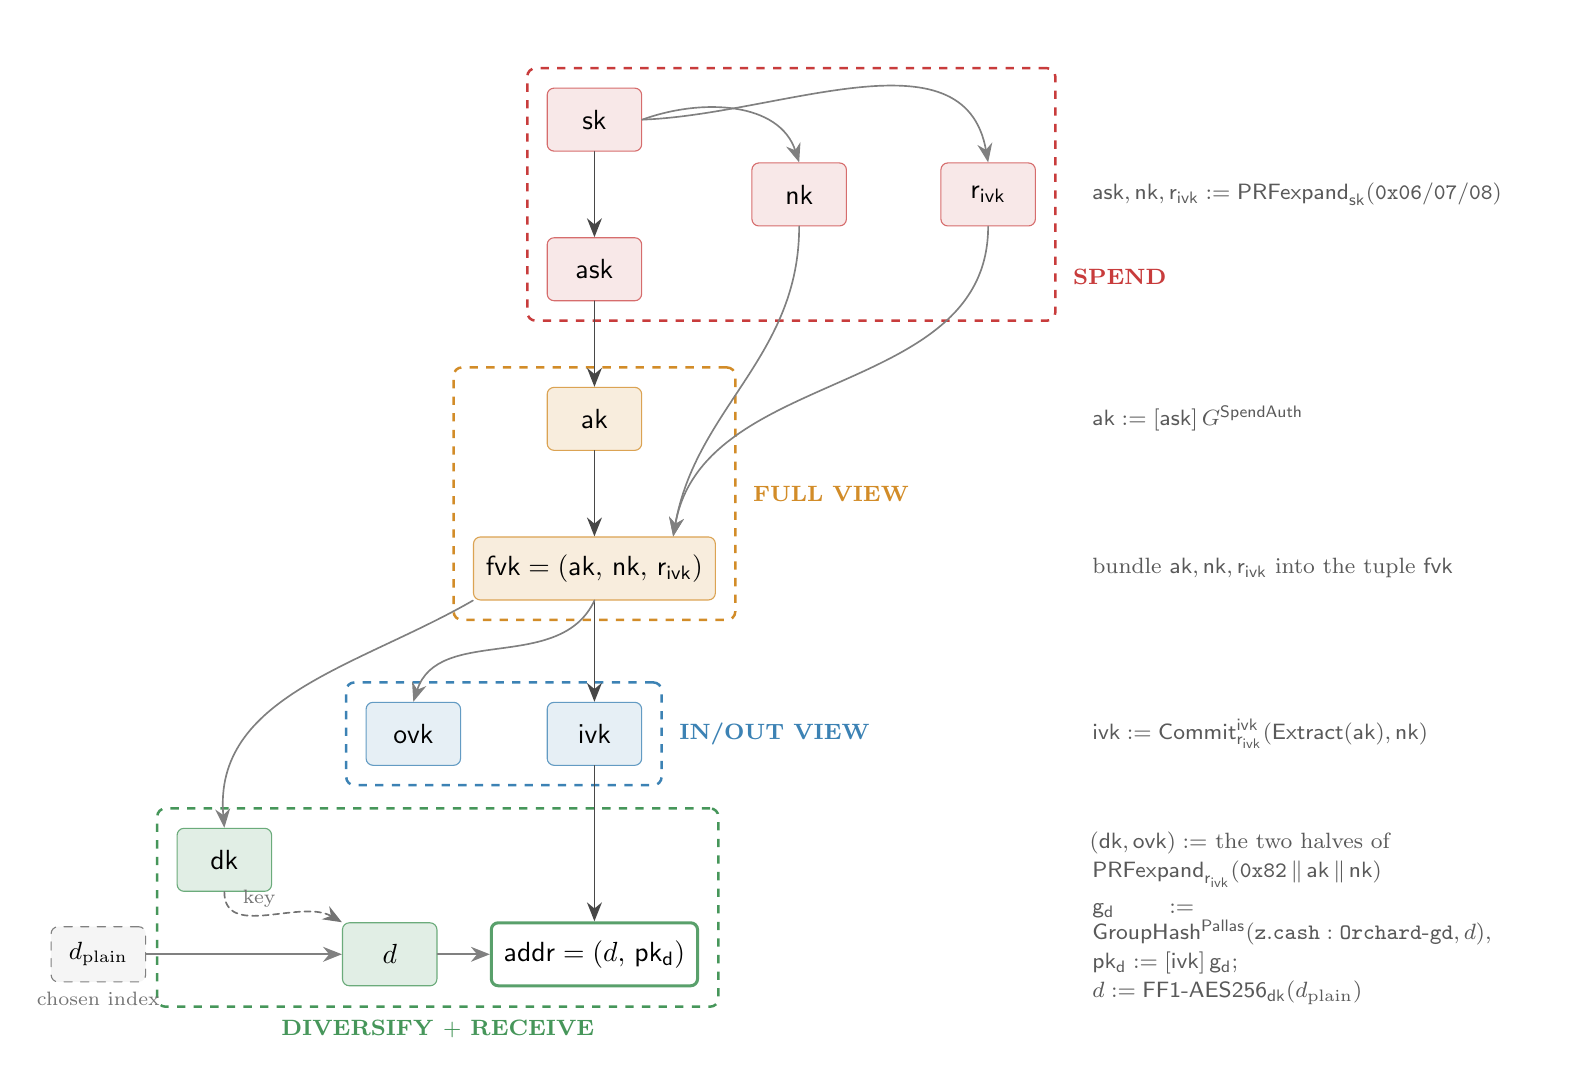
\begin{tikzpicture}[
  >={Stealth[length=2.4mm,width=1.9mm]},
  line cap=round, line join=round,
  box/.style={draw, rounded corners=2.5pt, minimum height=8mm, minimum width=12mm, inner sep=4.5pt, align=center, font=\normalsize},
  spendn/.style={box, fill=tierspend!12, draw=tierspend!75},
  fulln/.style={box, fill=tierfull!16, draw=tierfull!80},
  inoutn/.style={box, fill=tierin!13, draw=tierin!80},
  recvn/.style={box, fill=tierrecv!16, draw=tierrecv!80},
  pubn/.style={box, fill=white, line width=1.1pt, draw=tierrecv!90},
  inputn/.style={box, fill=black!4, dashed, draw=black!50, font=\small, minimum height=7mm},
  spine/.style={->, semithick, black!72, rounded corners=4pt},
  fork/.style={->, semithick, black!50, rounded corners=5pt},
  keyedge/.style={->, semithick, dash pattern=on 2.2pt off 1.6pt, black!55, rounded corners=5pt},
  op/.style={font=\footnotesize, text=black!65, anchor=west, align=left, text width=57mm},
  note/.style={font=\scriptsize, text=black!55},
  tlab/.style={font=\footnotesize\bfseries, rotate=90, fill=white, inner sep=1.5pt},
  tlabh/.style={font=\footnotesize\bfseries, fill=white, inner sep=1.5pt},
]
\def\gx{6.2}

% ===== main spend->receive spine (x = 0) =====
\node[spendn] (sk)   at (0, 0)     {$\mathsf{sk}$};
\node[spendn] (ask)  at (0,-1.9)   {$\ask$};
\node[fulln]  (ak)   at (0,-3.8)   {$\aksym$};
\node[fulln]  (fvk)  at (0,-5.7)   {$\fvk=(\aksym,\,\nksym,\,\rivk)$};
\node[inoutn] (ivk)  at (0,-7.8)   {$\ivk$};
\node[pubn]   (addr) at (0,-10.6)  {$\mathsf{addr}=(d,\,\pkd)$};

% ===== spend-side secrets expanded from sk (top row, to the right) =====
\node[spendn] (nk)   at (2.6,-0.95) {$\nksym$};
\node[spendn] (rivk) at (5.0,-0.95) {$\rivk$};

% ===== outgoing viewing key: paired with ivk as in/out viewing =====
\node[inoutn] (ovk)  at (-2.3,-7.8) {$\ovk$};

% ===== diversifier key + address row (the FF1-AES256 formula is in the gutter) =====
\node[recvn]  (dk)   at (-4.7,-9.4) {$\dk$};
\node[inputn] (dpln) at (-6.3,-10.6) {$d_{\mathrm{plain}}$};
\node[recvn]  (d)    at (-2.6,-10.6) {$d$};

% ===== spine arrows =====
\draw[spine] (sk)  -- (ask);
\draw[spine] (ask) -- (ak);
\draw[spine] (ak)  -- (fvk);
\draw[spine] (fvk) -- (ivk);
\draw[spine] (ivk) -- (addr);

% sk expands to nk, rivk (to the right)
\draw[fork] (sk.east) to[out=20,in=108] (nk.north);
\draw[fork] (sk.east) to[out=2,in=100]  (rivk.north);

% ak, nk, rivk bundle into fvk; nk and rivk land exactly on their slot in the
% fvk tuple (positions measured from the label's own widths above)
\coordinate (fvknk)   at ($(fvk.north)+(\fvknkX,0)$);
\coordinate (fvkrivk) at ($(fvk.north)+(\fvkrivkX,0)$);
\draw[fork] (nk.south)   to[out=-90,in=80] (fvknk);
\draw[fork] (rivk.south) to[out=-90,in=80] (fvkrivk);

% the full viewing key derives all three sub-keys: ivk (spine), ovk, dk
\draw[fork] (fvk.south)      to[out=-115,in=72]  (ovk.north);
\draw[fork] (fvk.south west) to[out=-150,in=95]  (dk.north);

% diversifier: chosen index d_plain, keyed by dk, gives d, which enters addr
\draw[fork] (dpln) -- (d.west);
\draw[keyedge] (dk.south) to[out=-90,in=150] node[pos=0.6,above left=-0.5mm,note]{key} (d.north west);
\draw[fork] (d.east) -- (addr.west);

% ===== operation gutter, each line aligned with the box that step produces =====
\node[op] at (\gx,-0.95) {$\ask,\nksym,\rivk := \mathsf{PRFexpand}_{\mathsf{sk}}(\mathtt{0x06}/\mathtt{07}/\mathtt{08})$};
\node[op] at (\gx,-3.8)  {$\aksym := [\ask]\,G^{\mathsf{SpendAuth}}$};
\node[op] at (\gx,-5.7)  {bundle $\aksym,\nksym,\rivk$ into the tuple $\fvk$};
\node[op] at (\gx,-7.8)  {$\ivk := \CommitIvk_{\rivk}(\Extract(\aksym),\nksym)$};
\node[op] at (\gx,-9.4)  {$(\dk,\ovk) := $ the two halves of\\[1pt]
                          $\mathsf{PRFexpand}_{\rivk}(\mathtt{0x82}\,\|\,\aksym\,\|\,\nksym)$};
\node[op] at (\gx,-10.6) {$\gd := \GroupHash^{\Pallas}(\mathtt{z.cash:Orchard\text{-}gd},d)$,\\[1pt]
                          $\pkd := [\ivk]\,\gd$;\\[1pt]
                          $d := \mathsf{FF1\text{-}AES256}_{\dk}(d_{\mathrm{plain}})$};

\node[note, anchor=north] at (dpln.south) {chosen index};

% ===== capability tiers (background bands) =====
\begin{scope}[on background layer]
\node[draw=tierspend, dashed, line width=0.9pt, rounded corners=3pt,
      fit=(sk)(rivk)(ask)(nk), inner sep=7pt] (Tspend) {};
\node[draw=tierfull, dashed, line width=0.9pt, rounded corners=3pt,
      fit=(ak)(fvk), inner sep=7pt] (Tfull) {};
\node[draw=tierin, dashed, line width=0.9pt, rounded corners=3pt,
      fit=(ivk)(ovk), inner sep=7pt] (Tin) {};
\node[draw=tierrecv, dashed, line width=0.9pt, rounded corners=3pt,
      fit=(dk)(d)(addr), inner sep=7pt] (Trecv) {};
\end{scope}
% tier labels: rotated on the left edge, except the wide bottom one set below
\node[tlabh, text=tierspend, anchor=west] at ($(Tspend.east)+(1.5mm,-1.05)$) {SPEND};
\node[tlabh, text=tierfull, anchor=west]  at ($(Tfull.east)+(1.5mm,0)$)       {FULL VIEW};
\node[tlabh, text=tierin, anchor=west] at ($(Tin.east)+(1.5mm,0)$) {IN/OUT VIEW};
\node[tlabh, text=tierrecv, anchor=north] at ($(Trecv.south)+(0,-1mm)$) {DIVERSIFY \textmd{+} RECEIVE};
\end{tikzpicture}%
}
\caption{The Orchard key hierarchy as a capability ladder, read top to
bottom. Each arrow is a derivation; the right-hand gutter shows the
operation that produces the child from its parent(s). Not every edge is
one-way: the bundling edges ($\aksym,\nksym,\rivk$ into the tuple $\fvk$;
$d$ into the address) invert by projection, and the FF1 edge is a keyed
permutation the $\dk$ holder inverts --- the tiers are separated by the
one-way steps $\mathsf{sk}\to(\ask,\nksym,\rivk)$, $\ask\to\aksym$,
$\fvk\to(\ivk,\dk,\ovk)$, and $\ivk\to\pkd$. The $\dk$ and
$\ovk$ keys are the two halves of one $\mathsf{PRFexpand}_{\rivk}$ output (tag
$\mathtt{0x82}$, input $\aksym\|\nksym$); they play different roles and land
in different tiers --- $\ovk$ is the \emph{outgoing} viewing key, grouped with
the \emph{incoming} viewing key $\ivk$ as the IN/OUT viewing tier, whereas
$\dk$ is the \emph{diversifier} key, which sits in the address layer because
it generates diversified addresses. Concretely $d$ is the format-preserving
encryption $\mathsf{FF1\text{-}AES256}$ of a chosen index $d_{\mathrm{plain}}$
under the key $\dk$ (the dashed edge marks $\dk$ entering as the cipher key),
and $\pkd=[\ivk]\,\gd$, so the address binds both keys.
\emph{Every node is secret key material except the chosen index
$d_{\mathrm{plain}}$, the diversifier $d$, and the diversified address
(unshaded) --- the address $(d,\pkd)$, and with it $d$, is the only value
the protocol ever publishes} (shading marks tier membership, not secrecy) ---
in particular the viewing keys $\fvk$, $\ivk$, $\ovk$ are \emph{secret:}
``viewing''
names what they let the holder do, not that the protocol publishes them. Each dashed
tier holds a strictly weaker capability than the one above, so a holder may
receive a lower-tier key without gaining the powers above it. Drawn to
match Definition~\ref{def:keys}.}
\label{fig:keytree}
\end{figure}

The structure is a deliberate capability ladder (Figure~\ref{fig:keytree}),
each rung conferring strictly less power than the one above:

\begin{itemize}[leftmargin=*]
\item $\mathsf{sk}$ / $\ask$ --- \emph{spend}. Whoever holds $\ask$ can
authorise spends; it sits at the top and nothing below it can recover it.
\item $\fvk$ (hence $\ivk, \ovk$) --- \emph{see everything}. Detects
incoming notes (via $\ivk$, which recovers $\pkd$) and views outgoing notes
(via $\ovk$), but cannot spend, because deriving $\fvk$ from
$\mathsf{sk}$ is one-way.
\item $\ivk$ alone --- \emph{detect incoming}. Sufficient to recognise notes
addressed to the holder and scan the chain, nothing more --- the key suitable
for an always-online wallet server.
\item A diversified address $(d, \pkd)$ --- \emph{receive}. A public
handle anyone can pay; one $\ivk$ generates $2^{88}$ mutually unlinkable
addresses --- one per diversifier index (Definition~\ref{def:keys}),
practically inexhaustible --- all spendable by the same key.
\end{itemize}

Of these, only the diversified address is
\emph{public}. The viewing keys $\fvk, \ivk, \ovk$ are \emph{secret} key
material --- ``viewing'' names what they let the holder \emph{do} (see
transactions), not that one may publish them. Disclosing a viewing key
confers the corresponding visibility on the recipient --- every payment to
and from the wallet for $\fvk$, incoming payments only for $\ivk$,
outgoing only for $\ovk$ --- so the owner shares one only deliberately
(with an auditor, say) and otherwise guards it like any other secret. The ladder is useful precisely
because these capabilities are \emph{separable}: one can delegate
``see incoming'' ($\ivk$) without delegating ``see everything'' ($\fvk$),
and neither confers the ability to spend.

Two questions of motivation that the bare formulas do not answer. \emph{Why is $\ivk$
a commitment, $\CommitIvk_{\rivk}(\Extract(\aksym), \nksym)$, rather than a plain
hash?} Because $\ivk$ must both bind \emph{and} hide. It binds $\aksym$
(spend authority) and $\nksym$ (nullifier derivation) to one identity, and
check A7 below proves the linkage in-circuit by recomputing the commitment
from the witnessed $\aksym$, $\nksym$, $\rivk$ --- but binding alone a
collision-resistant hash would supply equally, and in-circuit recomputation
works for any hash (check A3 recomputes the unblinded Sinsemilla
$\mathsf{MerkleCRH}$; Sapling even proved its BLAKE2s-based
$\mathsf{CRH}^{\mathsf{ivk}}$ in-circuit). What the trapdoor $\rivk$ adds is
\emph{hiding}: the blinded $\ShortCommit$ is perfectly hiding, so $\ivk$ ---
and hence every public $\pkd = [\ivk]\gd$ --- reveals nothing about $\aksym$
and $\nksym$, whereas the unblinded Sinsemilla hash is only
collision-resistant (Theorem~\ref{thm:sinsemilla-cr}) with no one-wayness
claim. Hiding is what keeps the IN/OUT tier strictly below FULL VIEW: an
$\ivk$ holder, such as an always-online wallet server, cannot extract
$\nksym$ or $\aksym$.
\emph{Why is $\nksym$ separate from $\ask$?} So that the owner can delegate the
capability to compute nullifiers (which a viewing key needs to determine which
of the holder's notes are already spent) \emph{without} conferring the ability to
spend --- the viewing key holds $\nksym$ but never $\ask$.
\FloatBarrier
\subsection{Representation of a note: notes and note commitments}\label{sec:notes}

The first requirement is to represent a note such that it stays invisible
on-chain yet provable by its owner. The protocol therefore never places the note on the
chain at all; it publishes only a hiding commitment to it.

\begin{definition}[Orchard note]\label{def:note}
An Orchard \emph{note} --- the private object representing one unit of value ---
is a tuple
\[
\mathbf{n} := (\mathsf{addr},\, v,\, \rho,\, \psi,\, \rcm),
\]
where $\mathsf{addr} := (d, \pkd)$ is the recipient's diversified address;
$v \in \{0, \dots, 2^{64} - 1\}$ is the value in zatoshi;
$\rho \in \F_{p_{\Pallas}}$ is a per-note uniqueness seed;
$\psi \in \F_{p_{\Pallas}}$ is randomness the sender fixes through the note
seed $\mathsf{rseed}$, from which it is derived deterministically
(\S\ref{sec:noteenc}); and
$\rcm \in \F_{p_{\Vesta}}$ is the commitment trapdoor.
\end{definition}

The protocol never publishes the note itself. What it records on-chain is its
\emph{note commitment}
\[
\cmsym := \NoteCommit_{\rcm}\bigl(\gd^\star \,\|\, \pkd^\star \,\|\, \mathrm{LE}_{64}(v) \,\|\, \mathrm{LE}_{255}(\rho) \,\|\, \mathrm{LE}_{255}(\psi)\bigr) \;\in\; \Ep(\F_{p_{\Pallas}}),
\]
a commitment that is \emph{perfectly hiding} (the chain learns nothing
about $\mathsf{addr}, v, \rho, \psi$ from $\cmsym$) and
\emph{computationally binding} (the sender cannot later claim the
commitment was to a different note). These are precisely the two properties
of a commitment scheme from the \emph{Crypto Guide}; here the scheme is
Sinsemilla (\S\ref{sec:sinsemilla}), chosen because it is inexpensive to
recompute \emph{inside the circuit}, which the spender must do. The chain
stores $\cmx := \Extract(\cmsym) \in \F_{p_{\Pallas}}$, the
$x$-coordinate of the commitment point, because the Merkle tree consumes a field element.

The three address-related quantities appearing in $\NoteCommit$ are the
key material that \S\ref{sec:orchard-keys} defines: the diversifier
$d \in \{0,1\}^{88}$, the diversified base
$\gd \in \Ep(\F_{p_{\Pallas}})$ (the per-address generator
$\GroupHash^{\Pallas}(\mathtt{z.cash:Orchard\text{-}gd}, d)$), and the
transmission key $\pkd = [\ivk]\,\gd \in \Ep(\F_{p_{\Pallas}})$ that
identifies the recipient; the address is $\mathsf{addr} = (d, \pkd)$.
Recall the $\star$-encoding from \S\ref{sec:prelim-curve}: $\gd^\star,
\pkd^\star \in \{0,1\}^{256}$. The $\NoteCommit$ input is the bit-string
concatenation ($\|$) of these point encodings with the little-endian
integer encodings $\mathrm{LE}_{64}(v) \in \{0,1\}^{64}$ and
$\mathrm{LE}_{255}(\rho), \mathrm{LE}_{255}(\psi) \in \{0,1\}^{255}$.

The choice of fields is as follows. $\mathsf{addr}$ and $v$ are the note's
content. $\rho$ and $\psi$ exist solely to render the eventual nullifier
unique and unpredictable; their role becomes apparent only in
\S\ref{sec:nullifier}: a note carries
randomness whose purpose is downstream.

\subsection{Proof of ownership of \emph{some} valid note: the commitment tree}\label{sec:tree}

The second requirement is to prove the spent note is valid without revealing
which note. When Alice spends, she must convince the network that
the note she is spending is a valid note that someone actually created;
otherwise she could spend a note she invented. On a transparent chain this
is trivial: the output is present in the UTXO set. But Alice must prove
it \emph{without revealing which note}, because revealing the note would
deanonymise the payment.

The network maintains one append-only Merkle tree whose leaves are
\emph{every note commitment ever published}, in creation order. Alice proves
\emph{membership}: a Merkle authentication path from her leaf $\cmx$ to a
root the network trusts. Inside the circuit the path is a private witness
(check~A3), so the verifier learns that her note is one of the leaves but not
which one; the anonymity set is the entire tree.

\begin{definition}[Orchard commitment tree]\label{def:tree}
The Orchard \emph{note commitment tree} is an append-only Merkle tree of
fixed depth $32$ (so up to $2^{32}$ notes). Leaves are $\cmx$ values in
creation order. The parent of a left child $\ell$ and right child $r$ at
layer $\ell'$ is
\[
\mathsf{MerkleCRH}^{\mathsf{Orchard}}_{\ell'}(\ell, r) := \mathsf{ShortHash}_{\mathtt{z.cash:Orchard\text{-}MerkleCRH}}(\mathrm{LE}_{10}(\ell') \,\|\, \mathrm{LE}_{255}(\ell) \,\|\, \mathrm{LE}_{255}(r)) \in \F_{p_{\Pallas}},
\]
a layer-tagged Sinsemilla short hash (Definition~\ref{def:sinsemilla-commit})
of the $10 + 255 + 255 = 520$-bit message --- $52$ ten-bit chunks, the same
$\mathrm{LE}$-encoded input convention as $\CommitIvk$ and $\NoteCommit$
(leaves $\cmx$, internal nodes, and the root all live in $\F_{p_{\Pallas}}$).
Appending a block's note commitments yields a new root: the root of the tree
after block $h$ is the \emph{anchor} of block $h$ (a single field element),
so every main-chain block defines exactly one anchor. A spend proves
membership against the anchor of any main-chain block, and all Actions of one
bundle prove against a single shared anchor (\S\ref{sec:netverify}).
\end{definition}

Every node is a single base-field element by necessity, not convention. The
spender recomputes this hash layer by layer \emph{inside} the Action circuit to
prove membership (check~A3 of \S\ref{sec:action-stmt}), and that circuit is
arithmetic over $\F_{p_{\Pallas}}$: every wire carries one such field element.
A curve-point node would carry two coordinates and an on-curve constraint at
each of the $32$ layers; reducing each node to its $x$-coordinate halves the
path data the circuit threads and removes that bookkeeping. This is precisely
why $\mathsf{MerkleCRH}$ ends in $\Extract$: $\Sinsemilla$ yields a point, and
$\Extract$ returns it to the field, so that each layer's output is directly the
next layer's input and the one hash composes all the way to the root. Dropping
the $y$-coordinate is harmless here (\S\ref{sec:prelim-curve}): the tree uses
each node only as a binding digest, never to recover a child point, and a
collision in the $x$-coordinate still reduces to one in $\Sinsemilla$
(Theorem~\ref{thm:sinsemilla-cr}).

Two design details are significant. The tag carries the layer
index $\ell'$ so that a path at one height cannot replay at another.
And empty leaf positions take an ``uncommitted'' sentinel value
$2$: the choice is not arbitrary --- at $x = 2$ the curve equation gives
$y^2 = 2^3 + 5 = 13$, and $13$ is a non-square modulo both Pasta primes (the
\emph{Math Guide} verifies this), so $2$ is not the $x$-coordinate of any
Pallas point, hence can never equal a valid $\cmx$ and can never be silently
confused with a genuine commitment.

\paragraph{Derivation of the authentication path.}
Alice's commitment occupies a fixed \emph{position} $\mathsf{pos}$ --- its
index in creation order --- which her wallet records when it detects the note
(\S\ref{sec:noteenc}). Fix an anchor of any block at or after the one that
mined her note, and let $n$ be the number of leaves in that block's tree. The
authentication path of leaf $\mathsf{pos}$ against that anchor consists of
one node per level: writing $\mathsf{pos} = b_{31} \cdots b_1 b_0$ in binary,
the level-$i$ ancestor of her leaf is a left child when $b_i = 0$ and a right
child when $b_i = 1$, and the path's level-$i$ entry is that ancestor's
\emph{sibling} in the tree of size $n$ (Figure~\ref{fig:merklepath}).
Check~A3 reverses the construction: starting from $\cmx$ it combines the
running node with one path entry per level --- placing the node on the side
$b_i$ dictates (left when $b_i = 0$, right when $b_i = 1$) and the sibling
opposite --- and asserts that the final value equals the public anchor; the
bits $b_i$ and the siblings stay inside the witness.

Each entry is one of two kinds. When $b_i = 1$ the sibling subtree lies to
the \emph{left} of her leaf: it spans commitments older than hers, so every
one of its positions is filled --- a \emph{complete} subtree --- and, because
the tree appends only on the right, its root is final and identical at every
anchor. When $b_i = 0$ the
sibling subtree lies to her \emph{right}, and its value depends on the
anchor: its root hashes the commitments it holds at size $n$, with positions
not yet filled taking the uncommitted sentinel $2$; a sibling subtree still
entirely empty at size $n$ contributes a per-level constant, the sentinel
folded up through the layer-tagged hash. The path is therefore a
deterministic function of $\mathsf{pos}$ and the first $n$ public leaves, and
of nothing else; the only secret is which leaf is hers.

In practice the wallet neither rebuilds the path from the leaves on each
spend nor retains the whole tree. As it scans, it appends every published
$\cmx$ --- its own and everyone else's --- but keeps only what a future path
needs: the nodes from each of its own notes up to the root, the
complete-subtree roots flanking those paths, and one \emph{checkpoint} per
block; the rest it prunes (this is the design of librustzcash's
\textsf{shardtree}). It marks its note's position the moment trial decryption
succeeds (\S\ref{sec:noteenc}). A checkpoint stores merely the position of
that block's last leaf, equivalently the leaf count $n$ --- the size that
fixes the block's anchor; the anchor itself is recomputed from the retained
nodes on demand, never stored.

To produce the path for a spend against a chosen block, the wallet descends
its retained tree to the marked leaf and, on the way back to the root, reads
off each sibling subtree's root: a complete subtree contributes its stored
root, a subtree lying wholly beyond the leaf count $n$ contributes the
per-level empty root, and the single subtree straddling position $n$ is
rehashed from its retained nodes. The leaf count enters only as this cutoff
--- every position $\ge n$ counts as empty --- so one retained tree
reproduces the path against any block it has checkpointed.

\begin{figure}[htbp]
\centering
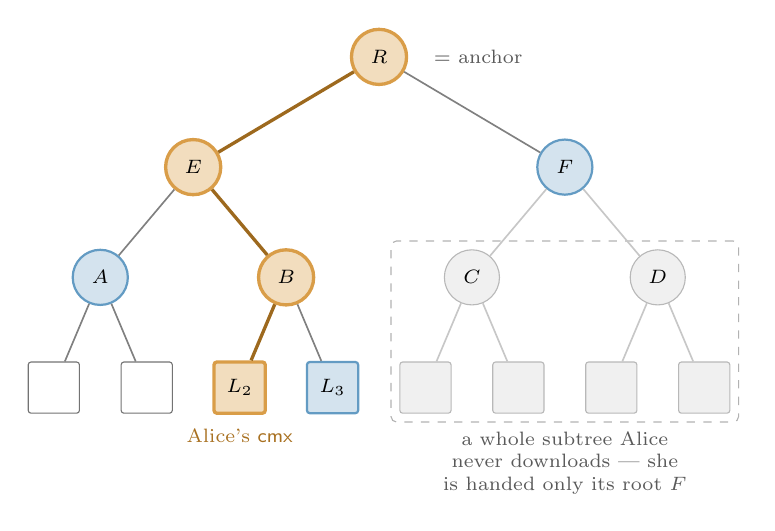
\begin{tikzpicture}[x=1.18cm,y=1.4cm,
  >={Stealth[length=2mm]},
  lf/.style={draw, rounded corners=1pt, minimum size=6.5mm, inner sep=0pt},
  nd/.style={draw, circle, minimum size=7mm, inner sep=0pt, font=\scriptsize},
  route/.style={fill=tierfull!30, draw=tierfull!85, very thick},
  sibl/.style={fill=tierin!22, draw=tierin!80, thick},
  near/.style={draw=black!55, fill=white},
  faded/.style={draw=black!28, fill=black!6},
  ed/.style={black!50, semithick},
  red/.style={draw=tierfull!75!black, very thick},
  fed/.style={black!22, semithick},
  lab/.style={font=\scriptsize, text=black!65},
]
\node[lf,near]  (L0) at (0,0) {};
\node[lf,near]  (L1) at (1,0) {};
\node[lf,route] (L2) at (2,0) {\scriptsize$L_2$};
\node[lf,sibl]  (L3) at (3,0) {\scriptsize$L_3$};
\node[lf,faded] (L4) at (4,0) {};
\node[lf,faded] (L5) at (5,0) {};
\node[lf,faded] (L6) at (6,0) {};
\node[lf,faded] (L7) at (7,0) {};
\node[nd,sibl]  (A) at (0.5,1) {$A$};
\node[nd,route] (B) at (2.5,1) {$B$};
\node[nd,faded] (C) at (4.5,1) {$C$};
\node[nd,faded] (D) at (6.5,1) {$D$};
\node[nd,route] (E) at (1.5,2) {$E$};
\node[nd,sibl]  (F) at (5.5,2) {$F$};
\node[nd,route] (R) at (3.5,3) {$R$};
\draw[ed]  (E)--(A); \draw[ed] (B)--(L3); \draw[ed] (R)--(F);
\draw[ed]  (A)--(L0); \draw[ed] (A)--(L1);
\draw[fed] (F)--(C); \draw[fed] (F)--(D);
\draw[fed] (C)--(L4); \draw[fed] (C)--(L5);
\draw[fed] (D)--(L6); \draw[fed] (D)--(L7);
\draw[red] (L2)--(B); \draw[red] (B)--(E); \draw[red] (E)--(R);
\node[lab, below=0.6mm of L2, text=tierfull!80!black] {Alice's $\cmx$};
\node[lab, anchor=west] at ($(R.east)+(2mm,0)$) {$=\ $anchor};
\begin{scope}[on background layer]
\node[draw=black!30, dashed, rounded corners=2pt, fit=(C)(D)(L4)(L5)(L6)(L7), inner sep=3pt] (fbox) {};
\end{scope}
\node[lab, anchor=north, align=center, text width=4.4cm] at (fbox.south) {a whole subtree Alice never downloads --- she is handed only its root $F$};
\end{tikzpicture}
\caption{Computation of a Merkle authentication path (drawn at depth $3$; Orchard's
tree has depth $32$). The leaves are the public note commitments $\cmx$, in
order. Alice's note sits at leaf $L_2$ (orange); to prove it is in the tree she
must compute the authentication path of $L_2$, then recompute the bold route
from $L_2$ up to the root $R$ --- the \emph{anchor} --- folding in, at each
level, the sibling hash beside it: that path is $L_3, A, F$ (blue).
Efficiency is the only reason not to hash
the whole tree: a far subtree enters her path solely through its single root
(here $F$), so she never downloads its leaves (faded) --- the
$\mathsf{GetSubtreeRoots}$ shortcut that lets even a freshly restored wallet
witness a years-old note.}\label{fig:merklepath}
\end{figure}

Nothing above requires Alice to have been online: the inputs are public, so a
freshly restored wallet rebuilds the same state by replaying the chain's note
commitments. Nor need it touch all $2^{32}$ positions, and here the tree's
structure earns its keep. Cut the tree at half its depth. Below the cut lie
the \emph{shards} --- the height-$16$ subtrees, $2^{16}$ leaves apiece, up to
$2^{16}$ of them --- and above it a height-$16$ \emph{cap} whose own leaves are
the shard roots (librustzcash sets the shard height to half the tree depth,
$32/2 = 16$). A leaf's $32$ siblings divide along the same cut: the low $16$
(levels $0$ through $15$) lie inside its own shard, and the high $16$ (levels
$16$ through $31$) are cap nodes, each the root of a subtree spanning whole
shards. The two halves reach Alice by entirely different routes, and that
asymmetry is the economy of the scheme.

Her own shard she must hash from leaves. Its $16$ low siblings are the
within-shard subtrees of the descent above --- complete to her left, straddling
or empty to her right --- so she scans that shard's commitments block by block,
her own and everyone else's, and folds them; this is the one subtree whose
$2^{16}$ leaves she handles individually. Every \emph{other} shard she takes as
a single $32$-byte root. The cap's leaves are exactly those roots, which a light
server streams one per completed shard ($\mathsf{GetSubtreeRoots}$); Alice folds
them upward with the same layer-tagged $\mathsf{MerkleCRH}$, one application per
cap level --- the upper half of the tree's $32$ layers --- and reads her high
siblings off the result (Figure~\ref{fig:merklepath} is the toy-depth analogue:
the faded subtree enters only through its root $F$). A shard that does not yet
exist --- the empty right of the cap --- contributes the per-level empty
constant rather than a download, and her own shard she holds from leaves whether
or not it has completed, so she never needs its root from the server. Her
level-$16$ sibling is thus a neighbouring shard's root, and each sibling above
it a fold of $2, 4, 8, \dots$ roots she already holds.

A concrete case fixes the shape. Let Alice's note be the \emph{last} leaf of the
newest shard $k$. Below the cut, all $16$ low siblings are complete left
subtrees tiling the shard's earlier $2^{16} - 1$ positions, so she ingests
essentially the whole shard. Above the cut, the cap's right side is empty --- no
shard succeeds $k$, so those siblings are the empty constant --- while its left
side folds the roots of shards $0, \dots, k-1$, each supplied by
$\mathsf{GetSubtreeRoots}$. Stitching the halves --- her leaf folds up to the
shard-$k$ root, which folds up the cap to the anchor --- gives the full
$32$-level path.

The $2^{16}$ throughout bounds the cap's \emph{capacity} --- $2^{32}$ leaves over
$2^{16}$ per shard --- not Alice's traffic. She fetches one root per shard that
actually exists, $\lceil n/2^{16} \rceil$ of them: a few hundred at present tree
sizes, and growing by one every $2^{16}$ outputs. The whole history above her
shard thus arrives as a few kilobytes of roots in place of millions of leaves.
She performs the fold \emph{locally}, never asking a server for one particular
note's path, which would reveal which note is hers; the finished path is the
private witness of check~A3, and only the anchor is public.

\paragraph{Anchor choice as the tree grows.}
By the time Alice's transaction reaches a block, the live tree has advanced
past her chosen anchor. This costs nothing: appending leaves creates new
roots and alters no old one, so the anchor still names one fixed historical
tree, her path still folds to exactly that root, and check~A3 asserts exactly
that equality --- collision resistance of the layer-tagged hash
(\S\ref{sec:sinsemilla}) makes a path to that root for a non-member
infeasible. Consensus accepts the anchor of \emph{any} main-chain block from
Orchard activation onward (NU5, mainnet block $1{,}687{,}104$); there is no
sliding window, so proving is fully decoupled from broadcasting --- Alice
need not race the chain tip. The one recency caveat runs in the opposite
direction: a reorganisation can strike the anchoring block from the main
chain, invalidating the anchor and forcing her to rebuild the transaction;
anchoring at least $100$ blocks deep (Zcash's reorg limit) avoids this
entirely. Deployed wallets nonetheless anchor close to the tip, by
deliberate choice rather than necessity. The anchor's tree is the anonymity
set in which check~A3 conceals the spent note --- the proof reveals only that
the note is \emph{some} leaf committed by that anchor --- so the most recent
admissible anchor, naming the largest such tree, maximises that set, while an
idiosyncratically old or deep anchor would instead fingerprint the spender.
\textsf{librustzcash} accordingly selects the most recent block it has
checkpointed that lies at least a fixed number of confirmations behind the tip
(by default, per ZIP-315, $3$ confirmations for notes the wallet produced
itself and $10$ for notes received from third parties), trading a sliver of
reorg robustness for set size and uniformity. Consensus mandates none of this;
it is wallet policy. Nor is an old anchor a soundness hole: membership in an older,
smaller tree implies the note was committed even earlier, which is precisely
what Alice must establish --- the nullifier (\S\ref{sec:nullifier}), not the
anchor, prevents a second spend.

\subsection{Prevention of double-spending: nullifiers}\label{sec:nullifier}

The third requirement: to prevent Alice from spending the same note twice, without a
public registry of spent notes (which would leak exactly what is being
hidden). Each note yields a single deterministic
tag --- its \emph{nullifier} --- that appears only when its owner spends the note.
The network maintains a set of all revealed nullifiers and rejects any
repeat. The nullifier must satisfy two properties that pull in opposite directions:
it must be \emph{deterministic} (so the same note always
yields the same tag, making a second spend detectable) yet
\emph{unlinkable} (so that publishing it reveals nothing about which note
or address it came from).

\begin{definition}[Orchard nullifier]\label{def:nullifier}
For a note $\mathbf{n}$ with commitment $\cmsym$ and the owner's nullifier
key $\nksym$,
\[
\nfsym := \Extract\bigl(\bigl[\, F_{\nksym}(\rho) + \psi \,\bigr] G^{\mathsf{nf}} + \cmsym\bigr) \;\in\; \F_{p_{\Pallas}},
\]
where $F_{\nksym} : \F_{p_{\Pallas}} \to \F_{p_{\Pallas}}$ is a
circuit-efficient PRF (Poseidon over the Pallas base
field, the \emph{Crypto Guide}), $G^{\mathsf{nf}} := \GroupHash^{\Pallas}
(\mathtt{z.cash:Orchard}, \mathtt{K}) \in \Ep(\F_{p_{\Pallas}})$ is a fixed
nothing-up-my-sleeve Pallas generator (\S\ref{sec:prelim-curve}), the scalar $F_{\nksym}(\rho) +
\psi$ lives in $\F_{p_{\Pallas}}$ (a valid Pallas scalar because
$p_{\Pallas} < p_{\Vesta}$), and $\Extract$ takes the $x$-coordinate. (We
write $G^{\mathsf{nf}}$ for this base to distinguish it from the spend-auth
generator $G^{\mathsf{SpendAuth}}$ of \S\ref{sec:orchard-keys}.)
\end{definition}

We read the construction against the two requirements. Determinism: every
ingredient ($\nksym, \rho, \psi, \cmsym$) is fixed once the note exists, so
$\nfsym$ is a fixed function of the note --- spending it twice yields the same
$\nfsym$ twice, and the network rejects the second. Unlinkability: the term
$[F_{\nksym}(\rho) + \psi]\,G^{\mathsf{nf}}$ masks the commitment with a value that appears random
to anyone without $\nksym$, so no one can tie the published $\nfsym$ back
to $\cmsym$ or to the address (this is where the note's $\rho$ and $\psi$ perform their function). The security properties:

\begin{itemize}[leftmargin=*]
\item \emph{No double-spend} (the Orchard Book calls this \emph{balance},
since double-spending is how one would create value): each note has exactly
one nullifier, and forging a colliding nullifier for a different note
reduces to DL on Pallas.
\item \emph{Spend unlinkability}: without $\nksym$, the published $\nfsym$
is unlinkable to the note or address, under the Decisional Diffie--Hellman
(DDH) assumption on Pallas --- that $([a]G, [b]G, [ab]G)$ is computationally
indistinguishable from $([a]G, [b]G, [c]G)$ for independent uniform
$a,b,c$ --- together with the PRF assumption on $F$.
\item \emph{Forward consistency (Faerie resistance)}: a freshly created
note takes as its uniqueness seed the nullifier of the note spent alongside it,
$\rho_{\mathrm{new}} := \nfsym_{\mathrm{old}}$; since the network already
guarantees nullifiers are unique, this forces every note's $\rho$ to be
globally unique, closing an attack from earlier designs in which forged
notes could be made to share a nullifier.
\end{itemize}
\subsection{Transmission and detection of a note: encryption, trial decryption, and synchronisation}\label{sec:noteenc}

The on-chain $\cmx$ conceals the note entirely, which leaves a question the
commitment alone does not resolve: how does the recipient learn of the note
with which they were paid? The sender must deliver the note to them, privately, over
the same public chain. Orchard achieves this with \emph{in-band secret
distribution}: every Action carries, beside its commitment, a ciphertext only
the recipient can open.

\paragraph{Encryption (sender side).} Alice holds Bob's address $(d, \pkd)$,
with $\pkd = [\ivk]\,\gd$ and $\gd = \GroupHash^{\Pallas}(\mathtt{z.cash:Orchard\text{-}gd}, d)$
(\S\ref{sec:orchard-keys}). She forms the \emph{note plaintext}
$\mathsf{np} = (\mathtt{0x02}, d, v, \mathsf{rseed}, \mathsf{memo})$, where the
$32$-byte $\mathsf{rseed}$ --- drawn uniformly at random, fresh for each output
note --- is the master randomness from which she derives the
note's $\rcm$, $\psi$, and the ephemeral secret $\mathsf{esk}$ below, and
$\mathsf{memo}$ is a fixed $512$-byte field of sender-chosen data. Each
derivation is one $\mathsf{PRFexpand}$ call keyed by $\mathsf{rseed}$,
distinguished by a leading domain-separator byte and taking
$\rho := \nfsym_{\mathrm{old}}$ (as $32$ little-endian bytes) as input ---
which binds the note's secret randomness to its Action:
\begin{align*}
\psi   &:= \mathrm{ToBase}\bigl(\mathsf{PRFexpand}_{\mathsf{rseed}}(\mathtt{0x09} \,\|\, \rho)\bigr) \in \F_{p_{\Pallas}}, \\
\rcm   &:= \mathrm{ToScalar}\bigl(\mathsf{PRFexpand}_{\mathsf{rseed}}(\mathtt{0x05} \,\|\, \rho)\bigr) \in \F_{p_{\Vesta}}, \\
\mathsf{esk} &:= \mathrm{ToScalar}\bigl(\mathsf{PRFexpand}_{\mathsf{rseed}}(\mathtt{0x04} \,\|\, \rho)\bigr) \in \F_{p_{\Vesta}},
\end{align*}
where $\mathsf{esk}$ is redrawn under a fresh $\mathsf{rseed}$ in the rare event
it vanishes. She then runs a one-shot
Diffie--Hellman to a \emph{fresh} key:
\[
\mathsf{esk} \;\text{(above)}, \quad
\mathsf{epk} := [\mathsf{esk}]\,\gd, \quad
\mathsf{s} := [\mathsf{esk}]\,\pkd, \quad
K_{\mathrm{enc}} := \mathsf{KDF}(\mathsf{s}, \mathsf{epk}),
\]
and seals the plaintext under an AEAD (ChaCha20-Poly1305),
$C_{\mathrm{enc}} := \mathsf{Enc}_{K_{\mathrm{enc}}}(\mathsf{np})$. The KDF is
BLAKE2b-256 with personalisation \texttt{Zcash\_OrchardKDF} over
$\mathsf{s}^\star \,\|\, \mathsf{epk}^\star$. Because
$\pkd = [\ivk]\gd$, Bob can reach the same secret from his side as
$[\ivk]\,\mathsf{epk} = [\ivk][\mathsf{esk}]\gd = [\mathsf{esk}]\pkd$, so,
beside the sender (who knows $\mathsf{esk}$), exactly the holder of $\ivk$
can recover $K_{\mathrm{enc}}$ from the published
$(\mathsf{epk}, C_{\mathrm{enc}})$. A second ciphertext
$C_{\mathrm{out}}$, sealed under the \emph{outgoing cipher key}
$\mathsf{ock} := \mathrm{BLAKE2b\text{-}256}(\texttt{Zcash\_Orchardock},\
\ovk \,\|\, \cvsym^{\mathsf{net}} \,\|\, \cmx \,\|\, \mathsf{epk})$ (points in
$\star$-encoding; $\cvsym^{\mathsf{net}}$ is the Action's net value
commitment, \S\ref{sec:value}), carries
$(\pkd, \mathsf{esk})$ so that the \emph{sender} --- or an auditor holding $\ovk$
--- can re-derive $\mathsf{s}$ and read the note as well; because $\mathsf{ock}$
binds the Action's own $\cvsym^{\mathsf{net}}$, $\cmx$, and $\mathsf{epk}$, a $C_{\mathrm{out}}$
cannot be transplanted onto another Action. The Action publishes
$(\mathsf{epk}, C_{\mathrm{enc}}, C_{\mathrm{out}})$ alongside
$\cvsym^{\mathsf{net}}, \nfsym, \rk, \cmx$, with $\rk$ the randomised
validating key (\S\ref{sec:redpallas}).

\paragraph{Trial decryption (recipient side).} Nothing on chain marks which
Action pays Bob, so his wallet \emph{trial-decrypts every} Orchard output: for
each it recomputes $\mathsf{s} := [\ivk]\,\mathsf{epk}$,
$K_{\mathrm{enc}} := \mathsf{KDF}(\mathsf{s}, \mathsf{epk})$, and
$\mathsf{np} := \mathsf{Dec}_{K_{\mathrm{enc}}}(C_{\mathrm{enc}})$. The AEAD tag
makes an incorrect guess fail cleanly (it returns $\bot$), so a successful open
\emph{is} the detection that the note was his. He then re-derives the full note
from $(d, v, \mathsf{rseed})$ --- taking $\rho := \nfsym_{\mathrm{old}}$ from the
same Action --- and performs the two checks that close the obvious forgeries:
(i)~that the sender formed the ephemeral key honestly, $[\mathsf{esk}]\gd = \mathsf{epk}$
for the $\mathsf{esk}$ re-derived from $\mathsf{rseed}$ (the ZIP-212 check,
defeating a mauled $\mathsf{epk}$); and (ii)~that the note is indeed the one
the Action committed on chain, $\Extract\big(\NoteCommit_{\rcm}(\ldots)\big) = \cmx$. Only
when both hold does he accept. A sender can therefore never make Bob accept a
note inconsistent with the commitment.

\paragraph{Wallet synchronisation, including from cold storage.} This is the
operation a wallet performs when it restores from a seed. From the account's
``birthday'' height it walks the chain forward and trial-decrypts every Action;
a light wallet does so against \emph{compact} blocks, which carry only the
first $52$ bytes of $C_{\mathrm{enc}}$ --- those covering the compact note
plaintext: the lead byte $\mathtt{0x02}$ ($1$ byte), $d$ ($11$ bytes), $v$
($8$ bytes), and $\mathsf{rseed}$ ($32$ bytes) --- together with
$\mathsf{epk}$, $\cmx$, and the Action's nullifier $\nfsym$, which the
light wallet needs twice: it supplies $\rho := \nfsym_{\mathrm{old}}$ for
the $\cmx$ recomputation that detects the note, and it is the source of
the chain's nullifier set against which spentness is checked below. The
wallet records each note that opens \emph{with its leaf
position} --- the index at which it appended its $\cmx$, read directly off the
block --- and that position is precisely what the commitment tree of
\S\ref{sec:tree} consumes: the wallet \emph{marks} the position in its shard
tree and can then build the note's authentication path on demand, by the
root-only assembly described there, without replaying every commitment. To
determine which recovered notes remain spendable it additionally requires
$\nksym$: it computes each note's nullifier (\S\ref{sec:nullifier}) and discards
those whose nullifier already appears in the chain's nullifier set. The end
state is a set of unspent notes, each with a value, a position, an
authentication path, and a nullifier --- exactly what the Action prover of
\S\ref{sec:orchard-walkthrough} consumes.

\subsection{Conservation of value: value commitments and the binding signature}\label{sec:value}

The fourth requirement: to guarantee that a transaction creates no value, while
concealing every amount. The instrument is the additive homomorphism of
Pedersen commitments (the \emph{Crypto Guide}): commit to each amount, and
verify that the commitments \emph{sum} to the publicly declared net flow --- the
individual values remain hidden, while their balance is publicly verifiable.

\begin{definition}[Net value commitment]\label{def:cv}
Each Action commits to its own value change with a Pedersen commitment
\[
\cvsym^{\mathsf{net}} := [\,v_{\mathrm{old}} - v_{\mathrm{new}}\,]\,V^{\mathsf{Orchard}} + [\rcv]\,R^{\mathsf{Orchard}} \;\in\; \Ep(\F_{p_{\Pallas}}),
\]
where $v_{\mathrm{old}}$ is the spent value, $v_{\mathrm{new}}$ the created
value, $\rcv \in \F_{p_{\Vesta}}$ the commitment randomness (a Pallas
scalar), and
$V^{\mathsf{Orchard}} := \GroupHash^{\Pallas}(\mathtt{z.cash:Orchard\text{-}cv}, \texttt{"v"})$,
$R^{\mathsf{Orchard}} := \GroupHash^{\Pallas}(\mathtt{z.cash:Orchard\text{-}cv}, \texttt{"r"})
\in \Ep(\F_{p_{\Pallas}})$ are nothing-up-my-sleeve points
(\S\ref{sec:prelim-curve}), hence independent Pallas generators.
\end{definition}

The spender draws each $\rcv$ uniformly at random and afresh for every Action,
at the moment of bundle assembly. In contrast to the note's $\rcm$, $\psi$, and
$\mathsf{esk}$ --- all derived deterministically from the note seed
$\mathsf{rseed}$ (\S\ref{sec:noteenc}) --- $\rcv$ belongs to no note and is never
transmitted; its uniformity and secrecy are precisely what make
$\cvsym^{\mathsf{net}}$ hiding, and what keep the aggregate $\mathsf{bsk}$
introduced below known only to the transaction author.

We now apply the homomorphism. Summing over the $m$ Actions in a transaction,
\[
\sum_{i=1}^{m} \cvsym^{\mathsf{net},i} = \Bigl[\textstyle\sum_i (v_{\mathrm{old},i} - v_{\mathrm{new},i})\Bigr] V^{\mathsf{Orchard}} + [\mathsf{bsk}]\,R^{\mathsf{Orchard}}, \qquad \mathsf{bsk} := \sum_i \rcv_i \;\in\; \F_{p_{\Vesta}}.
\]
If the transaction is balanced, the bracketed value-component equals the
publicly declared net flow $v_{\mathrm{balance}}^{\mathsf{Orchard}}$ (a
signed field of the transaction; by convention a positive value is net value
flowing \emph{out} of the Orchard pool --- paying fees or transparent
outputs, say).
The network subtracts the declared part,
\[
\mathsf{bvk} := \sum_i \cvsym^{\mathsf{net},i} - [\,v_{\mathrm{balance}}^{\mathsf{Orchard}}\,]\,V^{\mathsf{Orchard}} \;\in\; \Ep(\F_{p_{\Pallas}}),
\]
and \emph{if and only if} the transaction balances, the
$V^{\mathsf{Orchard}}$-component cancels and $\mathsf{bvk} = [\mathsf{bsk}]\,
R^{\mathsf{Orchard}}$ is a public key whose secret $\mathsf{bsk}$ the
transaction author knows. Proving knowledge of that secret --- via a
\emph{binding signature} under key $\mathsf{bvk}$ --- is precisely
proving that the accounts balance, with no amount revealed. The binding
signature is RedPallas (\S\ref{sec:redpallas}) instantiated on the base
$R^{\mathsf{Orchard}}$, the value-commitment randomness base, distinct from
the spend-authorisation base $G^{\mathsf{SpendAuth}}$. A single signature
over the whole transaction (concretely, over the ZIP-244 \emph{sighash} below)
additionally binds all its Actions together, so that
no one can remove or transplant any of them.

\paragraph{The transaction digest (ZIP-244).} The message both Orchard
signatures sign --- the \emph{sighash} --- is not the raw transaction but a
non-malleable digest of it, which ZIP-244 assembles as a tree of personalised
$\mathrm{BLAKE2b\text{-}256}$ hashes, one node per transaction component. Its
root is
\[
\mathsf{sighash} := \mathrm{BLAKE2b\text{-}256}\bigl(\texttt{ZcashTxHash\_} \,\|\, \mathsf{branchid},\ d_{\mathrm{hdr}} \,\|\, d_{\mathrm{trans}} \,\|\, d_{\mathrm{Sap}} \,\|\, d_{\mathrm{Orch}}\bigr),
\]
where $\mathsf{branchid}$ is the $4$-byte identifier of the active network
upgrade --- so a signature is valid only on the fork it was made for --- and
each $d_\bullet$ is a personalised digest of one pool's data, an absent pool
hashing the empty string. A purely shielded Orchard payment leaves the
transparent and Sapling branches empty, and then the $\mathsf{sighash}$
coincides with the transaction identifier itself.

The Orchard branch commits to the entire bundle,
\[
d_{\mathrm{Orch}} := \mathrm{BLAKE2b\text{-}256}\bigl(\texttt{ZTxIdOrchardHash}, d_{\mathrm{C}} \,\|\, d_{\mathrm{M}} \,\|\, d_{\mathrm{N}} \,\|\, \mathsf{flagsOrchard} \,\|\, \mathrm{LE}_{64}(v_{\mathrm{balance}}^{\mathsf{Orchard}}) \,\|\, \mathsf{anchor}\bigr),
\]
through three digests that partition every Action's fields: the \emph{compact}
$d_{\mathrm{C}}$ over $\nfsym$, $\cmx$, $\mathsf{epk}$ and the first $52$ bytes
$C_{\mathrm{enc}}[0{:}52]$; the \emph{memo} $d_{\mathrm{M}}$ over the $512$-byte
$C_{\mathrm{enc}}[52{:}564]$; and the \emph{non-compact} $d_{\mathrm{N}}$ over
$\cvsym^{\mathsf{net}}$, $\rk$, the tail $C_{\mathrm{enc}}[564{:}]$ and
$C_{\mathrm{out}}$. Folding in every Action's $\nfsym$, $\cmx$,
$\cvsym^{\mathsf{net}}$, $\rk$ and ciphertexts beside the shared
$\mathsf{flagsOrchard}$, balance and $\mathsf{anchor}$, the $\mathsf{sighash}$
pins the exact bundle: no Action can be transplanted into another transaction
nor any field altered without breaking it. The SpendAuthSig under each $\rk$
and the binding signature under $\mathsf{bvk}$ both sign this single value.

\subsection{Authorisation of the spend: RedPallas}\label{sec:redpallas}

One capability remains: the spender must prove that they are \emph{authorised}
to spend the note --- that they hold $\ask$ --- and must do so without
linking this spend to any other spend by the same key. RedPallas, a
re-randomisable Schnorr signature, provides exactly this.

It is the Schnorr template of the \emph{Crypto Guide} on Pallas, with hash
$H^*$ (BLAKE2b-512 reduced mod $p_{\Vesta}$). The novel ingredient is
\emph{key re-randomisation}: the spender draws a randomiser
$\alpha \in \F_{p_{\Vesta}}$ uniformly at random, fresh for every Action
(RedPallas's $\mathsf{GenRandom}$: hash $80$ uniform bytes with $H^*$, which
makes $\alpha$ statistically uniform on $\F_{p_{\Vesta}}$), and sets
\[
\rsk := \ask + \alpha \;\in\; \F_{p_{\Vesta}}, \qquad \rk := \aksym + [\alpha]\,G^{\mathsf{SpendAuth}} = [\rsk]\,G^{\mathsf{SpendAuth}} \;\in\; \Ep(\F_{p_{\Pallas}}).
\]
The spender publishes the \emph{randomised} validating key $\rk$, not the
real $\aksym$, and signs with $\rsk$. Because $\alpha$ is fresh per spend,
$\rk$ is uniformly random and unlinkable across spends, yet remains a valid
key for the underlying authority. The circuit enforces that
$\rk$ is a re-randomisation of the witnessed $\aksym$ (check A6) and that
this $\aksym$ is the key bound into the note's address (check A7),
so that a valid Action proves the spender knows $\ask$ --- without ever
revealing $\aksym$.

\subsection{A single shielded payment, end to end}\label{sec:orchard-walkthrough}

The components now assemble into a transaction. Consider Alice paying Bob $5$
ZEC ($v = 5 \cdot 10^{8}$ zatoshi) from a note worth $5$ ZEC. The unit of shielded transfer is an
\emph{Action}, which simultaneously spends one old note and creates one new
note (a deliberately fixed shape that conceals whether a given Action is
``really'' a spend, an output, or both). This payment is one Action.

\paragraph{1. Bob hands Alice an address.} Bob derives a diversified
address $(d, \pkd)$ from his $\ivk$ (\S\ref{sec:orchard-keys}) and gives it
to Alice. It reveals nothing and is unlinkable to his other addresses.

\paragraph{2. Alice builds the Action.} Alice owns an old note
$\mathbf{n}_{\mathrm{old}}$ worth $5$ ZEC, whose commitment $\cmx_{\mathrm{old}}$
is a leaf of the tree. She:
\begin{itemize}[leftmargin=*]
\item computes its nullifier $\nfsym_{\mathrm{old}}$
(\S\ref{sec:nullifier}) --- she will publish this to retire the note;
\item constructs Bob's new note $\mathbf{n}_{\mathrm{new}} := (\mathsf{addr}_{\mathrm{Bob}}, 5 \cdot 10^{8}, \rho_{\mathrm{new}}, \psi_{\mathrm{new}}, \rcm_{\mathrm{new}})$
with $\rho_{\mathrm{new}} := \nfsym_{\mathrm{old}}$, and its commitment
$\cmx_{\mathrm{new}}$ (\S\ref{sec:notes});
\item forms the value commitment $\cvsym^{\mathsf{net}}$ with
$v_{\mathrm{old}} - v_{\mathrm{new}} = 5 \cdot 10^{8} - 5 \cdot 10^{8} = 0$ (\S\ref{sec:value});
\item selects a randomiser $\alpha$ and forms $\rk$ (\S\ref{sec:redpallas});
\item reads off a recent anchor and her note's Merkle path
(\S\ref{sec:tree}).
\end{itemize}

\paragraph{3. Alice proves the Action statement.} She runs the Halo 2
prover on the relation of \S\ref{sec:action-stmt}, with public inputs
$(\mathsf{anchor}, \cvsym^{\mathsf{net}}, \nfsym_{\mathrm{old}}, \rk,
\cmx_{\mathrm{new}})$ and her note, keys, path, and randomness as private
witness. The proof attests, in one shot and revealing nothing: the old note
is in the tree (A3), its nullifier follows correctly (A5), she is
authorised to spend it (A6, A7), the spent and created notes are well-formed (A1, A2), and
the value commitment is consistent (A4).

\paragraph{4. Alice assembles and signs the transaction.} She encrypts
$\mathbf{n}_{\mathrm{new}}$ to Bob (so that only Bob, via his $\ivk$, can detect
and open it; \S\ref{sec:noteenc}), attaches a SpendAuthSig under $\rk$, and signs the whole
bundle with the binding signature under $\mathsf{bvk}$ (\S\ref{sec:value}),
which proves balance; both signatures sign the ZIP-244 transaction sighash,
welding the Action into this transaction.

\paragraph{5. The network verifies.} Consensus checks: it recognises the anchor;
$\nfsym_{\mathrm{old}}$ is not already in the nullifier set
(no double-spend); the Halo 2 proof verifies; the SpendAuthSig verifies
under $\rk$; the binding signature verifies under the recomputed
$\mathsf{bvk}$ (balance). If all pass, it adds $\nfsym_{\mathrm{old}}$ to the
nullifier set and appends $\cmx_{\mathrm{new}}$ as a new tree leaf.

\paragraph{6. Bob receives.} Scanning with his $\ivk$, Bob trial-decrypts
the ciphertext (\S\ref{sec:noteenc}), recovers $\mathbf{n}_{\mathrm{new}}$, and now owns a $5$-ZEC
note he can later spend by repeating the entire procedure. The chain has gained
one nullifier and one commitment; an observer learns that \emph{an} Orchard
payment occurred and nothing else --- not sender, recipient, or amount.

That sequence constitutes the entire protocol. The formal Action statement below
is precisely the list of the in-circuit checks step 3 invokes.

\subsection{What a node verifies, without ever observing the note}\label{sec:netverify}

Note that none of the previous subsection involved the \emph{network}. A
validating node holds no viewing key, cannot trial-decrypt, and so never learns
the sender, recipient, or amount of any Action. What it \emph{can} do is confirm
that the hidden data is internally consistent --- and for that it relies entirely
on the proof, not on the note.

What the node receives is an Orchard \emph{bundle}, the unit into which the
v5 transaction format (ZIP-225) groups all Orchard data: the per-Action
public fields; one anchor shared by every Action in the bundle; a
\emph{single} aggregate Halo~2 proof covering all of the bundle's Actions;
and one SpendAuthSig per Action. The declared net flow
$v_{\mathrm{balance}}^{\mathsf{Orchard}}$ and the binding signature appear
once per bundle, and the flags $\mathsf{enableSpends}$,
$\mathsf{enableOutputs}$ are likewise bundle-level fields. Using only the
public fields
$(\mathsf{anchor}, \cvsym^{\mathsf{net}}, \nfsym_{\mathrm{old}}, \rk, \cmx)$ of
each Action, a node checks:
\begin{itemize}[leftmargin=*]
\item the bundle's \emph{Halo 2 proof} of the Action statement (\S\ref{sec:action-stmt})
--- this forces each spent note of nonzero witnessed value to be a genuine
tree leaf (a zero-value dummy spend skips the membership check by A3's
gate, by design), the nullifiers and new commitments to follow correctly,
and the keys to align;
\item the \emph{anchor} is a Merkle root the node has seen on its accepted main
chain (\S\ref{sec:tree});
\item $\nfsym_{\mathrm{old}}$ is \emph{not already} in the nullifier set --- the
one check that cannot sit inside a single proof, because it concerns the global
history (this prevents a double-spend);
\item the \emph{spend-authorisation signature} verifies under $\rk$ and the
\emph{binding signature} under the recomputed $\mathsf{bvk}$
(\S\S\ref{sec:value}--\ref{sec:redpallas}), settling authority and balance.
\end{itemize}
If every Action passes, the node performs the two state changes of step 5
--- recording each $\nfsym_{\mathrm{old}}$, appending each
$\cmx_{\mathrm{new}}$ --- which permit the next spender to prove membership
and make a second spend of the same note fail. Thus the SNARK together with the two signatures
enforces a payment's validity, never the inspection of the note: the node
confirms that the accounts balance and that no one forged anything \emph{while
learning nothing about the note itself}. This is the precise sense in which the
knowledge soundness of the Action SNARK (\S\ref{sec:e2e-sec}) performs all the
work --- the network trusts the proof exactly because a real witness extractably
backs a valid one.

\subsection{The Action statement, formally}\label{sec:action-stmt}

\begin{definition}[Orchard Action statement, NU5/NU6]\label{def:action}
The Action SNARK proves, with public inputs
\[
(\mathsf{anchor},\, \cvsym^{\mathsf{net}},\, \nfsym_{\mathrm{old}},\, \rk,\, \cmx,\, \mathsf{enableSpends},\, \mathsf{enableOutputs})
\]
and the note, keys, Merkle path, randomiser $\alpha$, and the
value-commitment trapdoor $\rcv$ as private witness, the conjunction:

\medskip\noindent
\textbf{[A1] Old-note commitment integrity} --- the spent note is
well-formed:
\[
\cmsym_{\mathrm{old}} = \NoteCommit_{\rcm_{\mathrm{old}}}\!\bigl(\gd_{\mathrm{old}}^\star \| \pkd_{\mathrm{old}}^\star \| \mathrm{LE}_{64}(v_{\mathrm{old}}) \| \mathrm{LE}_{255}(\rho_{\mathrm{old}}) \| \mathrm{LE}_{255}(\psi_{\mathrm{old}})\bigr)
\]
--- or $\NoteCommit$ returns $\bot$, the specification's escape hatch for
Sinsemilla's incomplete-addition exceptions (the remark following this
definition).

\noindent
\textbf{[A2] New-note commitment integrity}, with $\rho_{\mathrm{new}} := \nfsym_{\mathrm{old}}$:
$\Extract\bigl(\NoteCommit_{\rcm_{\mathrm{new}}}(\ldots)\bigr) \in \{\cmx, \bot\}$
(with $\Extract(\bot) := \bot$) --- the created note is well-formed
and its uniqueness seed chains to the spent note's nullifier (Faerie resistance).

\noindent
\textbf{[A3] Membership, gated by $v_{\mathrm{old}}$} --- the spent note is
a real leaf: recomputing the Merkle root from $\Extract(\cmsym_{\mathrm{old}})$
up the witness path of length $32$ gives $\mathsf{root}$, and
$v_{\mathrm{old}} \cdot (\mathsf{root} - \mathsf{anchor}) = 0$. (The gate by
$v_{\mathrm{old}}$ permits a zero-value ``dummy'' spend to skip the membership
check, which is how an Action pads with no real input.)

\noindent
\textbf{[A4] Net-value commitment integrity} --- the amounts are consistent
and in range: with witnessed $(\mathrm{magnitude}, \mathrm{sign})$,
$v_{\mathrm{old}} - v_{\mathrm{new}} = \mathrm{magnitude} \cdot \mathrm{sign}$,
$\cvsym^{\mathsf{net}} = [v_{\mathrm{old}} - v_{\mathrm{new}}] V^{\mathsf{Orchard}} + [\rcv] R^{\mathsf{Orchard}}$,
$v_{\mathrm{old}}, v_{\mathrm{new}} \in [0, 2^{64})$, $\mathrm{sign} \in \{-1,+1\}$.

\noindent
\textbf{[A5] Nullifier integrity} --- the published nullifier is indeed this
note's:
\[
\nfsym_{\mathrm{old}} = \Extract\bigl([F_{\nksym}(\rho_{\mathrm{old}}) + \psi_{\mathrm{old}}]\, G^{\mathsf{nf}} + \cmsym_{\mathrm{old}}\bigr).
\]

\noindent
\textbf{[A6] Spend authority} --- the published key is a re-randomisation of
the note owner's: $\rk = \aksym + [\alpha] G^{\mathsf{SpendAuth}}$.

\noindent
\textbf{[A7] Address integrity} --- the keys, address, and nullifier key all
belong to one identity:
$\ivk = \bot$, or
$\ivk = \CommitIvk_{\rivk}(\Extract(\aksym), \nksym)$ and
$\pkd_{\mathrm{old}} = [\ivk] \gd_{\mathrm{old}}$.

\noindent
\textbf{[A8] / [A9] Spend / output gating}:
$v_{\mathrm{old}} \cdot (1 - \mathsf{enableSpends}) = 0$ and
$v_{\mathrm{new}} \cdot (1 - \mathsf{enableOutputs}) = 0$. The transaction
builder sets these bundle-level flags; consensus rules constrain them
(coinbase transactions, for instance, must set $\mathsf{enableSpends} = 0$).
\end{definition}

A1, A2, and A7 take the specification's $\bot$-weakened forms because the
circuit cannot exclude Sinsemilla's incomplete-addition exceptional cases;
the relation proved is the disjunction, not the plain conjunction. The
weakening costs only a negligible soundness term: producing a $\bot$ case
is itself a non-trivial DL relation among the $\GroupHash$ generators (the
closing sentence of the proof of Proposition~\ref{prop:sins-cr}), so no
efficient prover exhibits one.

Each of A1--A7 is one entry from the four-requirement map of
\S\ref{sec:orchard-problem}: A1--A2 represent notes, A3 proves membership,
A5 (with the chain's nullifier set) prevents double-spending, A4 conserves
value, and A6--A7 authorise the spender; A8--A9 stand outside the map as
consensus-level gating constraints. This is the relation
$\Rel_{\mathsf{Orchard}}$. Every Action is an instance of it; Halo~2
produces one aggregate proof \emph{per bundle}, covering all of the
bundle's Actions, while each Action carries its own SpendAuthSig.
\S\ref{sec:circuit} sketches how the Action circuit arithmetises this relation,
and \S\ref{sec:e2e-sec} shows how soundness of the relation yields the
protocol's security properties.
\subsection{The Action circuit: arithmetisation of the relation}\label{sec:circuit}

The Action statement of \S\ref{sec:action-stmt} is a \emph{relation}; what Alice
actually executes is a \emph{circuit} that proves membership in it in zero
knowledge. Halo~2 (the \emph{Halo~2 Guide}) proves satisfiability of a fixed
PLONKish circuit, so the task of the application layer is to encode the
conjunction A1--A9 as one such circuit --- the \emph{Action circuit}, identical
for every Action --- supplied the note, keys, Merkle path, randomiser $\alpha$, and the
value-commitment trapdoor $\rcv$ as private witness. We sketch this encoding here; the gate-level
details appear in the \emph{halo2 Book} and the \emph{Orchard Book}.

We assemble the circuit from a small set of reusable \emph{gadgets} (``chips''),
each a pre-wired block of custom gates and lookups realising one operation. The
Orchard designers \emph{chose} the primitives so that these gadgets are inexpensive under
PLONKish arithmetisation; this motivates the use of Sinsemilla and Poseidon
rather than a bit-oriented hash. How any such gadget is \emph{built} --- how
its gates, lookups, and cell assignments are declared, and how synthesis
turns the filled columns into the polynomials the proof commits to --- is
the subject of the \emph{Halo~2 Guide}'s section ``From statement to
circuit''; here we describe what each gadget enforces.

\paragraph{The ECC gadget.} Implements the Pallas group law with the
\emph{complete} addition formulas (no edge-case failures; the
\emph{Math Guide}), together with variable- and fixed-base scalar
multiplication (the former a double-and-add ladder of incomplete-addition
rounds finished by a complete tail, the latter using precomputed fixed-base
tables; the $j$-invariant-$0$ endomorphism serves only the recursion layer's
endoscaling, not this circuit) and
on-curve witnessing. It realises every group operation in the statement:
$\aksym = [\ask]\,G^{\mathsf{SpendAuth}}$, the re-randomisation
$\rk = \aksym + [\alpha]\,G^{\mathsf{SpendAuth}}$ (A6), the transmission key
$\pkd = [\ivk]\,\gd$ (A7), the net value commitment
$\cvsym^{\mathsf{net}} = [\,v_{\mathrm{old}}-v_{\mathrm{new}}\,]\,V^{\mathsf{Orchard}} + [\rcv]\,R^{\mathsf{Orchard}}$
(A4), and the point $[\,F_{\nksym}(\rho)+\psi\,]\,G^{\mathsf{nf}} + \cmsym$ inside
the nullifier (A5).

\paragraph{The Sinsemilla gadget.} Implements $\Sinsemilla$
(\S\ref{sec:sinsemilla}) by realising its generator table $P[m]$ as a Halo~2
\emph{lookup} (the lookup argument of the \emph{Halo~2 Guide}): each $10$-bit
message chunk costs one table lookup and two incomplete additions. On it rest
the two composed commitment gadgets the Orchard Book names explicitly ---
\textsf{NoteCommit}, the in-circuit $\NoteCommit$ proving A1 and A2, and
\textsf{CommitIvk}, the in-circuit short commitment proving
$\ivk = \CommitIvk_{\rivk}(\Extract(\aksym),\nksym)$ in A7 --- each bundling the
Sinsemilla rounds with the bit-decomposition and canonicity checks of their field
inputs.

\paragraph{The Merkle-path gadget.} Stacks $32$ layer-tagged $\mathsf{MerkleCRH}$
hashes (themselves Sinsemilla short hashes, \S\ref{sec:tree}); at each layer a
conditional swap orders the running node and its witnessed sibling by one bit of
the leaf position, and the gadget asserts the recomputed root equal to the public
$\mathsf{anchor}$ --- check A3, gated by $v_{\mathrm{old}}$ so that a dummy spend
may skip it.

\paragraph{The Poseidon gadget.} Implements the Poseidon permutation
(\emph{Crypto Guide}), whose only non-linearity is $x \mapsto x^{5}$, to evaluate
the nullifier PRF $F_{\nksym}(\rho) = \mathsf{PoseidonHash}(\nksym,\rho)$ cheaply
in-circuit; its output feeds the ECC gadget for A5.

\paragraph{Decomposition, range, and boolean gadgets.} Lookup-based gadgets
split field elements into the bit-chunks the other gadgets consume and
range-check values: that $v_{\mathrm{old}}, v_{\mathrm{new}} \in [0, 2^{64})$ and
$\mathrm{sign} \in \{-1,+1\}$ (A4), and that point and field encodings are
canonical. (The flags $\mathsf{enableSpends}$, $\mathsf{enableOutputs}$ are
verifier-supplied public inputs --- ZIP-225's $\mathsf{flagsOrchard}$ byte
fixes them to bits outside the circuit --- and enter the circuit only
through the plain-gate products of A8--A9.)

\paragraph{Structure of the proof.} These gadgets compose into a single fixed
circuit whose native field is the Pallas base field $\F_{p_{\Pallas}}$ --- the
field in which Pallas coordinates reside, so that the ECC gadget runs natively ---
proved with the Halo~2 inner-product argument over the Pasta cycle. The
circuit uses $2^{11} = 2048$ rows (the \emph{Halo~2 Guide}'s circuit-size
exponent $k = 11$ --- not to be confused with Sinsemilla's chunk width
$k = 10$, Construction~\ref{const:sinsemilla}), with ten advice columns
beside the fixed columns and the Sinsemilla lookup table (the
\emph{Halo~2 Guide}). Every Action,
whatever it spends or creates, is one instance of this same circuit; a
bundle's Actions are proved together in one aggregate proof that a node
checks (\S\ref{sec:netverify}) from the public
inputs alone, and the accumulation machinery of the \emph{Halo~2 Guide} lets
a node verify many such proofs at amortised cost approaching that of a single
verification.

\section{End-to-end security: derivation of Orchard's properties from the SNARK}\label{sec:e2e-sec}

The Halo 2 SNARK on the Action relation, together with the algebraic structure of
the Orchard primitives, produces the security properties that render shielded
payments functional. We establish those connections below.

\subsection{Guarantees provided by a valid Action proof}\label{sec:what-proof-gives}

A SNARK $\pi$ accepted on public inputs
$(\mathsf{anchor}, \cvsym^{\mathsf{net}}, \nfsym_{\mathrm{old}}, \rk, \cmx, \ldots)$
testifies, with overwhelming probability, that the prover knows a
witness satisfying A1--A9. By knowledge soundness
of Halo 2 (the \emph{Halo 2 Guide}), an extractor can
recover this witness from any successful prover. The soundness-side
properties below (nullifier uniqueness, spend authority, balance) each
follow from one or more conjuncts of A1--A9 plus the algebraic properties
of the primitives; \S\ref{sec:sins-cr} first supplies the primitive
reduction those arguments share, and privacy rests instead on the zero
knowledge of the SNARK (\S\ref{sec:halo-zk}) together with the DDH,
Poseidon-PRF and KDF/AEAD assumptions that
Theorem~\ref{thm:orchard-e2e}(iv) adds.

\subsection{Reduction of Sinsemilla collision-resistance to DL on Pallas}\label{sec:sins-cr}

\begin{proposition}[Sinsemilla CR $\Leftarrow$ DL]\label{prop:sins-cr}
A collision $M \ne M'$ between messages of the same chunk count $\ell$
with $\Sinsemilla_D(M) = \Sinsemilla_D(M')$
yields a non-trivial DL relation among the generators
$\{P[0], \dots, P[2^k - 1]\}$.
\end{proposition}

\begin{proof}[Sketch]
Unfolding the Sinsemilla update (in the case no incomplete-addition
exception occurs), with $\ell$ the number of $k$-bit chunks:
\[
\Sinsemilla_D(M) = 2^\ell \cdot Q + \sum_{i=1}^{\ell} 2^{\ell - i} \cdot P[m_i].
\]
A collision gives $\sum_i 2^{\ell-i}(P[m_i] - P[m_i']) = 0$, i.e.\ a
non-trivial linear relation over $\F_{p_{\Vesta}}$ on the generators. Since
hash-to-curve modelled as a random oracle samples these independently,
finding such a relation is the multi-generator discrete-log relation
problem, and no efficient adversary produces one without solving DL (the
\emph{Crypto Guide} gives this reduction in its Pedersen-hash collision
analysis). For differing chunk counts $\ell \ne \ell'$, the unfolded
equality instead gives $(2^{\ell} - 2^{\ell'})\,Q + \sum_i \cdots =
\mathcal{O}$ with $2^{\ell} \not\equiv 2^{\ell'} \pmod{p_{\Vesta}}$ for all
admissible lengths, i.e.\ a non-trivial DL relation among $\{Q\} \cup
\{P[0], \dots, P[2^k - 1]\}$; since $Q$ is itself a $\GroupHash$ output
modelled as an independent random generator, this case reduces to DL
identically. The incomplete-addition exceptions are themselves
non-trivial DL relations among the same generators and so also
negligible.
\end{proof}

Sinsemilla CR is the primitive ingredient for note-commitment binding:
two distinct notes cannot share a commitment, so A1 and A2 are
genuine integrity statements about $\cmsym_{\mathrm{old}}$ and
$\cmsym_{\mathrm{new}}$. Combined with knowledge soundness, this entails
that the prover knows the specific opening of each commitment.

\subsection{Nullifier uniqueness}\label{sec:nf-unique}

\begin{proposition}[Nullifier uniqueness]\label{prop:nf-unique}
Two distinct notes $\mathbf{n} \ne \mathbf{n}'$ cannot share a nullifier
except with probability negligible in the DL hardness of Pallas (treating
Poseidon outputs as random scalars under the PRF assumption).
\end{proposition}

\begin{proof}[Sketch]
A collision $\nfsym(\mathbf{n}) = \nfsym(\mathbf{n}')$ in $x$-coordinate
gives
$[F_{\nksym}(\rho) + \psi] G^{\mathsf{nf}} + \cmsym = \pm([F_{\nksym}(\rho') + \psi'] G^{\mathsf{nf}} + \cmsym')$,
a non-trivial linear relation among $G^{\mathsf{nf}}, \cmsym, \cmsym'$.
Expanding $\cmsym, \cmsym'$ via their known openings (extracted by
knowledge soundness, or supplied by the adversary who forged the notes)
over the Sinsemilla generators and the blinding base $H_D$ turns this into
a known non-trivial DL relation among the independent $\GroupHash$ outputs
$\{G^{\mathsf{nf}}, Q, P[0], \dots, P[2^k - 1], H_D\}$ --- distinctness of
the notes forces some coefficient mismatch --- and producing such a
relation reduces to DL on Pallas as in Proposition~\ref{prop:sins-cr}.
\end{proof}

A5 (nullifier integrity) plus knowledge soundness ensures that
$\nfsym_{\mathrm{old}}$ in the public inputs is genuinely the nullifier of
some specific committed note, not an arbitrary value. The chain's
duplicate-nullifier rejection then prevents double-spending.

\subsection{RedPallas unforgeability and re-randomisation}\label{sec:redpallas-sec}

\begin{proposition}[RedPallas EUF-CMA $\Leftarrow$ DL]\label{prop:redpallas}
RedPallas is EUF-CMA-secure assuming DL on Pallas in the random-oracle
model. The re-randomisation extension preserves security: a forger that,
given $\aksym$ and signatures under re-randomised keys, produces a valid
signature under $\rk = \aksym + [\alpha]\, G^{\mathsf{SpendAuth}}$ for an
$\alpha$ of its own (possibly $\aksym$-dependent) choice yields a DL
solver for $\aksym$.
\end{proposition}

\begin{proof}[Sketch]
The standard forking argument (the \emph{Crypto Guide}, via the
Bellare--Neven general forking lemma) reduces a Schnorr forger to a DL adversary, and
it covers re-randomisation because RedPallas is key-prefixed: the
challenge $H^*(R \,\|\, \rk \,\|\, m)$ hashes the verification key, so
response-shifting cannot transport signatures between keys. The reduction
embeds the DL challenge as $\aksym := X$. It answers signing queries under
any $\rk_i = \aksym + [\alpha_i]\, G^{\mathsf{SpendAuth}}$ without knowing
any secret, via the honest-verifier zero-knowledge simulator with
random-oracle programming: sample $c, s$ uniformly, set
$R := [s]\, G^{\mathsf{SpendAuth}} - [c]\, \rk_i$, and program
$H^*(R \,\|\, \rk_i \,\|\, m) := c$, aborting on programming collisions
exactly as in the \emph{Crypto Guide}'s Schnorr EUF-CMA theorem. It then
forks the adversary at the forgery's critical query
$H^*(R^* \,\|\, \rk^* \,\|\, m^*)$, obtaining two accepting transcripts
that share $R^*$ --- and, since both forks share the critical query input,
the same $\rk^*$, hence the same $\alpha^*$ --- with distinct challenges;
$2$-special soundness extracts $\rsk^*$, the discrete logarithm of
$\rk^*$, and the output $\ask = \rsk^* - \alpha^*$, with $\alpha^*$ the
adversary-supplied randomiser, solves DL for $\aksym$. Separately, and
only for honest signer-chosen uniform $\alpha$: sampling $\alpha$ at
random and back-deriving $\aksym := \rk - [\alpha]\, G^{\mathsf{SpendAuth}}$
reproduces the view of $(\aksym, \alpha, \rk)$ exactly, so honest
re-randomisations are distributed as plain Schnorr keys --- the
unlinkability statement of the \emph{Crypto Guide}, which does not by
itself cover adversary-chosen $\alpha$.
\end{proof}

A6 (spend authority) plus knowledge soundness ensures the prover knows
$\alpha$ relating $\rk$ to $\aksym$; combined with the SpendAuthSig
under $\rk$ at the transaction layer, this enforces that the spender
knows $\ask$ corresponding to $\aksym$, hence to the address
$\pkd_{\mathrm{old}}$ via A7.

\subsection{Balance preservation via the Pedersen homomorphism}\label{sec:balance}

The combination of A4 (per-Action value commitment integrity), the
Pedersen homomorphism on $\cvsym^{\mathsf{net}}$, and the binding
signature on $\mathsf{bvk}$ gives end-to-end balance:

\begin{proposition}[Balance]\label{prop:balance}
Any accepted Orchard bundle has
$\sum_i (v_{\mathrm{old}, i} - v_{\mathrm{new}, i}) = v_{\mathrm{balance}}^{\mathsf{Orchard}}$
except with probability negligible in the DL hardness of the Pasta
curves in the random-oracle model (Vesta for the knowledge soundness of
the Action SNARK supplying the A4 openings; Pallas for the
binding-signature extraction and the independence of the
value-commitment bases).
\end{proposition}

\begin{proof}[Sketch]
By A4 and knowledge soundness, each $\cvsym^{\mathsf{net}, i}$ commits
to the true per-Action delta $v_{\mathrm{old}, i} - v_{\mathrm{new}, i}$.
The bundle sum $\sum_i \cvsym^{\mathsf{net}, i}$ equals $[\sum_i (v_{\mathrm{old}, i} - v_{\mathrm{new}, i})] V^{\mathsf{Orchard}} + [\sum_i \rcv_i] R^{\mathsf{Orchard}}$
by homomorphism. Consensus computes $\mathsf{bvk}$ and checks the
binding signature; a valid binding signature is a Fiat--Shamir proof of
knowledge of $\log_{R^{\mathsf{Orchard}}} \mathsf{bvk}$, so the forking
extraction in the proof of Proposition~\ref{prop:redpallas} recovers
$\mathsf{bsk}$ with $\mathsf{bvk} = [\mathsf{bsk}]\, R^{\mathsf{Orchard}}$;
combined with the openings extracted via A4, a non-zero
$V^{\mathsf{Orchard}}$-component of $\mathsf{bvk}$ would yield a
discrete-log relation between the independent bases $V^{\mathsf{Orchard}}$
and $R^{\mathsf{Orchard}}$, contradicting DL --- hence the value-component
equals $[v_{\mathrm{balance}}] V^{\mathsf{Orchard}}$ and the total value
flow matches the declared transparent balance.
\end{proof}

This is the fundamental conservation property: shielded transactions
cannot mint zatoshi out of nothing.

\subsection{Zero knowledge of the SNARK}\label{sec:halo-zk}

Halo 2 is statistical zero knowledge in the random-oracle model
(the \emph{Halo 2 Guide}'s zero-knowledge analysis). The simulator on input the instance
$(\mathsf{anchor}, \cvsym^{\mathsf{net}}, \nfsym_{\mathrm{old}}, \rk, \cmx, \ldots)$
operates as follows:
\begin{enumerate}[leftmargin=*]
\item Sample the Fiat--Shamir challenges $\theta, \beta, \gamma, y, x, x_1, x_2, x_3, x_4$
and the IPA challenges $u_1, \dots, u_{k}$ ($k = 11$ rounds, the
circuit-size exponent) uniformly, programming the
random oracle to return these on the relevant transcript prefixes.
\item Sample the final IPA scalar $a$ uniformly.
\item Use the freedom in the blinding terms $\ell_j, r_j$ (added at each
IPA round) and the polynomial blinders (added to each committed prover
polynomial: the advice columns in phase 1, the running products in phase 3,
and the quotient chunks in phase 4) to satisfy
the verifier's equations algebraically without knowing the witness.
\end{enumerate}
The resulting transcript is statistically indistinguishable from a real
proof; the only gap from perfect ZK is the random-oracle programming,
which a verifier that observes only the transcript cannot detect.

ZK supplies the proof's share of Orchard's privacy: the SNARK transcript
reveals nothing beyond the public inputs of each Action. That the published
data leak nothing further is a separate, computational matter: the
nullifier --- itself a public input (\S\ref{sec:nullifier}) --- hides its
note under the PRF security of Poseidon, and the $\mathsf{epk}$ and
ciphertexts published alongside the public inputs (\S\ref{sec:noteenc})
hide recipient and value under the DDH and KDF/AEAD assumptions that
Theorem~\ref{thm:orchard-e2e}(iv) adds.

\subsection{Composition of end-to-end soundness}\label{sec:e2e-snd}

The full SNARK soundness composes three ingredients:
\begin{itemize}[leftmargin=*]
\item \emph{PIOP soundness.} Schwartz--Zippel error per polynomial-identity
check, summed across constraints. For $\F = \F_{p_{\Pallas}}$ with
$|\F| \approx 2^{254}$ and constraint degree $\le d_{\max}$, the error
per check is $\le d_{\max}\, n / |\F| \approx d_{\max} \cdot 2^{-243}$
(the gate polynomial composes degree-$d_{\max}$ gates with column
polynomials of degree $n-1$, $n = 2^{11}$; a cheating prover's recombined
quotient $h \cdot Z_H$ has degree $< d_{\max} n$), overwhelmingly small.
\item \emph{PCS extractability.} Reduces to DL on the IPA curve
(the \emph{Halo 2 Guide}), with the accumulation analysis
(the \emph{Halo 2 Guide}) covering the deferred-MSM batching by which a
node amortises verification across proofs (\S\ref{sec:circuit}); the same
analysis would carry soundness across recursion, which Orchard's
deployment does not use.
\item \emph{Fiat--Shamir soundness in the ROM.} The \emph{Crypto Guide}'s
FS theorem covers $\Sigma$-protocols, losing roughly a factor $Q$ in the
prover's RO-query budget; for the $\log d$-round Halo~2 transcript the
naive multi-round analysis loses $q^{O(\log d)}$ (the \emph{Halo 2
Guide}), a bound vacuous at $Q = 2^{80}$. The negligible-error conclusion
rests on the tighter treatments the \emph{Halo 2 Guide} presents:
BCMS20's direct ROM+DL analysis, or Ghoshal--Tessaro's tight Fiat--Shamir
bound in the AGM.
\end{itemize}

Each step's soundness error is negligible at Orchard's parameters
($|\F| \approx 2^{254}$, $\lambda = 127$ under the
group-order-$\approx 2^{2\lambda}$ convention; effectively $\approx 126$
bits after the automorphism speedups, the \emph{Crypto Guide}); the union
bound across steps is itself negligible. Combined with the application-level reductions
(Propositions \ref{prop:sins-cr}--\ref{prop:balance}), the full chain
gives:

\begin{theorem}[Orchard end-to-end security, informal]\label{thm:orchard-e2e}
Under DL on both Pasta curves (Pallas for the application-level
primitives, Vesta for the IPA commitment) in the random-oracle model ---
and, for property (iv), additionally DDH on Pallas, the PRF security of
Poseidon (\S\ref{sec:nullifier}), and the KDF/AEAD securing the note
ciphertext (\S\ref{sec:noteenc}) --- no efficient adversary
can (i) produce an accepted Action without knowing a witness satisfying
A1--A9 --- in particular, any Action whose witnessed $v_{\mathrm{old}}$ is
nonzero must spend a genuine leaf of the commitment tree (zero-value dummy
spends, A3's gate, are accepted by design), (ii) cause two Actions to share
a nullifier without spending the same note twice, (iii) cause a bundle's
declared transparent balance $v_{\mathrm{balance}}^{\mathsf{Orchard}}$ to
differ from its true net value flow
$\sum_i (v_{\mathrm{old},i} - v_{\mathrm{new},i})$ --- in particular, to
exceed it, which would create value (Proposition~\ref{prop:balance}), or
(iv) link a published Action to any specific recipient or value beyond
what is explicit in the public inputs.
\end{theorem}

The four properties are, respectively, soundness of the Action SNARK,
nullifier uniqueness, balance preservation, and zero knowledge. The first
three reduce (informally) to DL on the Pasta curves in the ROM (Pallas
for the application-level reductions, Vesta for the IPA extraction). For
the fourth (privacy), the zero knowledge of the SNARK transcript is
statistical --- given the perfectly-hiding Pedersen and Sinsemilla
blinders and the random-oracle programming, it does not rest on DL ---
but full unlinkability of an Action additionally rests on the DDH
assumption on Pallas and the PRF security of Poseidon
(\S\ref{sec:nullifier}) and on the KDF/AEAD securing the note ciphertext
(\S\ref{sec:noteenc}), and is therefore computational. The asymmetry
within the proof itself is typical of the discrete-log SNARK family:
soundness is computational (a cheating prover is only \emph{bounded},
not impossible), whereas the zero knowledge of the transcript is
information-theoretic.

\section{The Zcash proof-system landscape}\label{sec:zcash}

This section closes with a survey of the proof systems Zcash has used across its
three generations of shielded payments. Concrete trade-offs drove each transition:
trusted setup risk, recursion compatibility, post-quantum
posture, and on-chain efficiency.

\subsection{Sprout (2016--present, deprecated)}

The original shielded protocol used a \emph{BCTV14} SNARK (Ben-Sasson,
Chiesa, Tromer, Virza) over the pairing-friendly curve BN254, with
constant-size proofs ($\sim 290$ bytes) and constant verification time. Its
parameters came from a per-circuit trusted setup: the 2016 ceremony, a
six-party multi-party computation that generated the BCTV14 proving and
verification keys for the fixed Sprout circuit, sound provided at least one
participant destroyed their secret share. Sprout demonstrated that
zk-SNARK shielded payments were feasible at scale, but it remained a
transitional design: the prover was slow, and the circuit hashed with
SHA-256 --- a bit-oriented hash whose boolean operations are non-native to
arithmetic constraints, hence costly in-circuit. Decisively, a flaw in
BCTV14 discovered in 2018 would have allowed undetected counterfeiting; the
pool was deprecated and shielded Sprout value was migrated to later pools.

\subsection{Sapling (2018--present)}

Sapling (the second network upgrade) replaced this stack with Groth16 --- $192$-byte
proofs, three-pairing verification --- over BLS12-381, with the embedded
curve Jubjub serving the in-circuit group operations and a Pedersen hash
serving the Merkle tree. The result was a far faster prover, a smaller
proof, and cheaper in-circuit hashing. Two structural limitations remained.
Groth16 still requires a per-circuit trusted setup --- the 2018 Sapling MPC,
whose universal first phase was the Powers of Tau ceremony with many
participants --- and no known elliptic-curve cycle extends BLS12-381, so the
proving system admits no efficient recursion.

\subsection{Orchard (2022--present, NU5)}

Orchard (NU5) replaced the Sapling stack with the Halo 2 / Pasta stack
developed in the \emph{Halo 2 Guide}. The principal choices are:
\begin{itemize}[leftmargin=*]
\item Halo 2: PLONKish PIOP, IPA-PCS, accumulation-friendly. No trusted
setup.
\item Pasta cycle: Pallas as the application curve, with Vesta as the
proving curve in the IPA layer. Designed for recursion.
\item Sinsemilla hash: an algebraic hash whose collision resistance reduces
to DL on Pallas --- an assumption the protocol already requires elsewhere
--- and whose chunk-table structure maps directly onto Halo~2's lookup
argument (\S\ref{sec:sinsemilla}).
\item Poseidon: serves the nullifier PRF (\S\ref{sec:nullifier}), where a
keyed in-circuit PRF rather than a CRH is required. Unlike Sinsemilla, its
security rests on cryptanalytic confidence in algebraic-attack resistance
rather than on a hardness assumption such as DL.
\end{itemize}

The shift followed a consistent design principle: ``transparent SNARK, recursion-ready''
constituted the design target, and the designers engineered the Pasta cycle to fit.

\subsection{Comparative summary}

\begin{table}[h]\centering\small
\begin{tabular}{@{}lccc@{}}
\toprule
& Sprout & Sapling & Orchard \\
\midrule
SNARK & BCTV14 & Groth16 & Halo 2 \\
Curve & BN254 & BLS12-381 + Jubjub & Pallas + Vesta \\
Trusted setup & Per-circuit (six-party MPC) & Per-circuit (large MPC) & None \\
Recursion-ready & No & No & Yes (via Pasta cycle) \\
Proof size & \textasciitilde 290 B & 192 B & \textasciitilde 5 kB (one Action) \\
Verification time & Constant (pairing) & Constant (3 pairings) & $O(\log n)$ amortised \\
\bottomrule
\end{tabular}
\caption{Three generations of Zcash shielded-payment proof systems.
Orchard verification: $O(\log n)$ amortised ($n = 2^{11}$ rows; per-proof
succinct checks, the linear MSM batched across proofs --- the \emph{Halo 2
Guide}).}\label{tab:zcash-history}
\end{table}

The proof size grew between Sapling and Orchard; this is the cost of
transparency (a one-Action bundle's proof occupies $2720 + 2272 = 4992$
bytes in the v5 encoding, including the $2\log_2 2^{11} = 22$ group
elements of the IPA rounds). The benefit, beyond the removal of trusted setup, is the
foundation for recursion: future generations (Tachyon, eventual rollup
designs) can build on Orchard's foundation without revisiting the
cryptographic stack.
\section{Post-quantum security of the deployed protocol}\label{sec:pq-orchard}

Every group-structured assumption in Theorem~\ref{thm:orchard-e2e} --- DL on
both Pasta curves and, for property (iv), DDH on Pallas --- falls to Shor's
algorithm in polynomial time on a cryptographically relevant quantum computer
(CRQC; the \emph{Crypto Guide}, \S``The quantum caveat: Shor's algorithm'');
the theorem's remaining assumptions, the PRF security of Poseidon and the
security of the KDF/AEAD, are symmetric and face only the generic speedups of
\S\ref{sec:pq-grover}. The productive question is therefore not \emph{whether} the
assumptions fail --- they all do, together --- but \emph{when the failure
matters}. We organise this section by \emph{reversibility}. A break is
\emph{retroactive} when data already recorded on chain becomes exploitable the
day the adversary exists: no later consensus change can help, because the data
is public and permanent. A break is \emph{prospective} when it requires a
validator to \emph{accept} a forged object after the adversary exists:
disabling the affected protocol before that day removes every future
acceptance event and mitigates the break completely. Deployed Orchard has
exactly one retroactive break (\S\ref{sec:pq-hndl}); everything else on its
assumption surface is prospective (\S\ref{sec:pq-integrity}) or faces only
generic quantum speedups (\S\ref{sec:pq-grover}).

Much of this section concerns design-stage material, so we make the epistemic
status of every forward-looking claim explicit, in one of three bins:
\emph{specified} (a published artifact pins the construction down, which we
cite), \emph{designed but unspecified} (an informal source describes the
design; we say what a specification would still need to fix), and \emph{open
problem} (no artifact exists). Claims about the deployed protocol instead cite
the implementation and the specification as elsewhere in this volume. Ground
truth for this section: \texttt{protocol.tex} and the ZIPs at \texttt{zips}
commit \texttt{c6b70358} (2026-07-05), and crate \texttt{orchard} at commit
\texttt{bef8a27e} (v0.14.0, 2026-06-16); we verified each cited artifact at
these commits.

\subsection{The retroactive break: harvest now, decrypt later against note
encryption}\label{sec:pq-hndl}

Each Action publishes the pair $(\mathsf{epk}, C_{\mathrm{enc}})$
(\S\ref{sec:noteenc}; crate \texttt{orchard},
\texttt{src/note\_encryption.rs}). Confidentiality of $C_{\mathrm{enc}}$ rests
on exactly one discrete-log-dependent link: the one-shot Diffie--Hellman on
Pallas between $\mathsf{esk}$ and $\pkd$ (protocol \S5.4.5.5; the
$\mathsf{esk}$ derivation is \texttt{src/note.rs}, the key agreement
\texttt{src/keys.rs}). The KDF and the AEAD above it are symmetric and are not
the weak layer (\S\ref{sec:pq-grover}).

A CRQC that knows a recipient's address $(d, \pkd)$ computes
\[
\ivk = \log_{\gd} \pkd
\]
by Shor --- one discrete logarithm for the lifetime of the address --- and then
runs the recipient's own trial-decryption loop of \S\ref{sec:noteenc} over the
recorded chain: for every Action, $[\ivk]\,\mathsf{epk}$ recovers
$K_{\mathrm{enc}}$, and the AEAD tag identifies which ciphertexts belong to the
address. The adversary obtains, for every note ever sent to that address, the
plaintext $(d, v, \mathsf{rseed}, \mathsf{memo})$: every amount, every memo,
the complete receiving history --- and equally every \emph{future} ciphertext
to the same address. Two limits bound the damage. First, $\ivk$ is a viewing
capability, not a spending one (\S\ref{sec:orchard-keys}): no spend authority
is conferred, and $\ask$ is not exposed. Second, the attack is keyed by the
address: without $(d, \pkd)$ the adversary has neither the base $\gd$ nor the
target $\pkd$, and the recorded chain reveals nothing further even to an
unbounded adversary (\S\ref{sec:pq-integrity}). ZIP-2005 records the same
boundary: the harvest-now-decrypt-later exposure requires ``both the
ciphertext \dots\ and the recipient address''.

The break is retroactive by construction. The pair
$(\mathsf{epk}, C_{\mathrm{enc}})$ is consensus data, replicated on every full
node forever; its secrecy was fixed at recording time by one specific DH
instance; any protocol upgrade alters only ciphertexts not yet created. An
adversary needs no quantum computer today --- only storage --- and every
Orchard output recorded since NU5 activation in 2022 is already in that
corpus.

\paragraph{Open problem: mitigation.} Nothing is deployed, and nothing is
specified, that protects even future ciphertexts. ZIP-2005 (Proposed) excludes
privacy by an explicit Non-requirement, states that the exposure persists for
all pools including Ironwood, and says only that mitigations for future
transfers are ``under consideration''. The tracking issues
(\texttt{zcash/zips\#1133}, open since 2022; \texttt{\#1134}, open since 2016)
carry discussion, not drafts; the \texttt{zips} repository at commit
\texttt{c6b70358} contains no occurrence of ML-KEM, Kyber, ML-DSA, or a
lattice scheme. A future hybrid key encapsulation would in any case protect
future outputs only; the recorded ciphertexts are unrepairable.

\subsection{Prospective breaks: the discrete-logarithm integrity
stack}\label{sec:pq-integrity}

The remainder of the assumption surface protects \emph{integrity}, and every
piece of it fails against the same adversary. The reductions of
\S\ref{sec:e2e-sec} each run equally well in reverse: the assumption a CRQC
falsifies is exactly the one the security proof consumes.

\begin{itemize}[leftmargin=*]
\item \emph{Sinsemilla binding.} Collision resistance reduces to the
discrete-log relation problem among the $\GroupHash$ generators
(Proposition~\ref{prop:sins-cr}). A CRQC computes every pairwise logarithm,
after which each Sinsemilla commitment opens to arbitrary messages: a second
note under an on-chain $\cmx$ (breaking balance through
\NoteCommit\ non-binding), a fabricated membership path under any anchor
(\S\ref{sec:tree}), and alternative pairs $(\aksym', \nksym')$ opening the
same \CommitIvk\ --- the Faerie-Gold-style Spendability attacks ZIP-2005
catalogues. A balance violation committed this way is bounded only by the
ZIP-209 turnstile and need not be detected at all.
\item \emph{Value commitments and the binding signature.} Binding of
$\cvsym^{\mathsf{net}}$ is the unknown discrete-log relation between
$V^{\mathsf{Orchard}}$ and $R^{\mathsf{Orchard}}$
(Definition~\ref{def:cv}, Proposition~\ref{prop:balance}); the binding
signature is Schnorr under DL in the ROM. Knowledge of
$\log_{V^{\mathsf{Orchard}}} R^{\mathsf{Orchard}}$ reopens any recorded or
fresh $\cvsym$ to any value and yields $\mathsf{bsk}$ for any target
$\mathsf{bvk}$: silent inflation, again turnstile-bounded (crate
\texttt{orchard}, \texttt{src/value.rs}).
\item \emph{RedPallas spend authorisation.} Unforgeability is DL in the ROM
(Proposition~\ref{prop:redpallas}). One logarithm --- of $\aksym$, or of any
published $\rk$ --- forges spend authorisation at will (crate
\texttt{orchard}, \texttt{src/primitives/redpallas.rs}); combined with the
next item it completes arbitrary theft.
\item \emph{IPA knowledge soundness.} The Action SNARK is sound under DL on
Vesta with Fiat--Shamir in the ROM (\S\ref{sec:e2e-snd}). A CRQC forges
accepting proofs of false Action statements: minting from nothing, spending
any commitment on chain, indistinguishable from honest proofs. This is the
single most concentrated failure point --- every other item's exploitation
route runs through it (crate \texttt{halo2\_proofs},
\texttt{src/poly/commitment.rs}).
\end{itemize}

\paragraph{Why forking in time is a complete mitigation.} Each attack above
must place a forged object --- a proof, a signature, a commitment opening ---
before a validator and have it \emph{accepted}, and acceptance happens at
current height under current consensus rules. Disabling the DL-dependent pools
before a CRQC exists removes every future acceptance event; transactions
already recorded were validated when the assumptions held and are never
re-adjudicated. The breaks are therefore fully prospective, with two residues.
Switch-off must precede the first forgery --- an attack landed in the exposure
window is not repaired afterwards (\S\ref{sec:pq-zip2005}) --- and honest
funds inside a disabled pool need some other way out, which is precisely the
problem ZIP-2005 exists to solve.

\paragraph{What the recorded chain does not leak.} The same recorded data that
becomes forgeable leaks no secrets, quantumly or otherwise. The value
commitment is perfectly hiding, so recorded $\cvsym$ values reveal nothing
about amounts even to an unbounded adversary (\S\ref{sec:value}). The
randomiser $\alpha$ is uniform, so recorded $\rk$ values and signatures carry
information-theoretically no linkage to $\aksym$ or $\ask$
(\S\ref{sec:redpallas-sec}). Proof transcripts are statistically simulatable
without the witness (\S\ref{sec:halo-zk}). Nullifiers are keyed by $\nksym$,
which never appears on chain (\S\ref{sec:nullifier}). Consequently a quantum
adversary who does not know a recipient's address learns nothing from the
recorded chain --- ZIP-2005 reaches the same conclusion --- and the sole
retroactive channel is the address-keyed decryption of \S\ref{sec:pq-hndl}.

\subsection{Primitives facing only generic speedups}\label{sec:pq-grover}

Two primitive families in Orchard carry no discrete-log structure. BLAKE2b
serves $\mathsf{PRFexpand}$ and with it every key and note-randomness
derivation (\S\ref{sec:orchard-keys}, \S\ref{sec:noteenc}), the KDF and the
outgoing cipher key, the RedPallas challenge hash, and the ZIP-244 sighash;
the ZIP-32 Orchard key tree is hardened-only, built entirely from these
derivations, with no elliptic-curve operation anywhere on the derivation path
(ZIP-32, Final; crate \texttt{orchard}, \texttt{src/zip32.rs}). Poseidon
serves the nullifier PRF, keyed by $\nksym$ (\S\ref{sec:nullifier};
\texttt{src/note/nullifier.rs}).

Against these, a quantum adversary gets generic speedups and nothing more ---
with the usual square-root caveat stated exactly. Grover search halves
effective preimage security (the \emph{Crypto Guide}, \S``The quantum caveat:
Shor's algorithm''): $2^{256}$ classical evaluations become
${\sim}2^{128}$ quantum ones, a margin the parameters absorb. For collisions
the picture is better still: the Brassard--H{\o}yer--Tapp $2^{n/3}$ algorithm
requires random access to a quantum memory of ${\sim}2^{92}$ bits at these
output sizes, and the best \emph{known} implementable generic quantum
collision attack remains the classical parallel one --- the assessment
ZIP-2005 adopts, flagged there as best-known rather than provably best.
Poseidon adds one honest caveat of its own: its PRF security is a
cryptanalytic heuristic with no standard-problem reduction, classically and
quantumly alike (\S\ref{sec:zcash}); a quantum adversary gains no identified
structural advantage, and since $\nksym$ stays off chain, recorded nullifiers
remain unlinkable either way.

The consequence is the load-bearing fact of the next subsection: the symmetric
backbone survives a discrete-log break intact. A seed holder can still prove,
by re-executing derivations, that their keys descend from their seed ---
ownership remains \emph{provable} after the assumption that made it
\emph{enforceable} has fallen.

\subsection{ZIP-2005: quantum recoverability for the Ironwood
pool}\label{sec:pq-zip2005}

ZIP-2005 (``Ironwood Quantum Recoverability'', Proposed; created 2025-03-31)
is the deployed-track response to the prospective breaks of
\S\ref{sec:pq-integrity}. It does not make Orchard quantum-secure and says so;
it arranges that funds survive the eventual switch-off.

\paragraph{Deployment.} Activation is bound to the NU6.3 network upgrade
(ZIP-258, Draft: consensus branch $\mathtt{0x37A5165B}$; Testnet activation
height $4134000$; Mainnet height not yet set at \texttt{zips} commit
\texttt{c6b70358}).
NU6.3 introduces the \emph{Ironwood pool}, carried by v6 transactions
(ZIP-229, Draft) and running Orchard with an updated Action circuit; the
scheduling follows the NU6.2 emergency circuit correction (ZIP-257, Final),
which is why the originally planned earlier deployment slipped. From
activation the legacy Orchard pool is sealed to spend-only: coinbase may carry
no Orchard-pool Actions, no new value may enter the pool
($v_{\mathrm{balance}}^{\mathsf{Orchard}} \ge 0$), and cross-address transfers
within it are disabled --- this last rule enforced by the height-selected
Action-circuit verifying key, the other two as ordinary consensus rules
(ZIP-258).

\paragraph{Mechanism.} Ironwood note plaintexts carry lead byte
$\mathtt{0x03}$ in place of $\mathtt{0x02}$, and for them the trapdoor
derivation changes from the deployed one --- domain-separated by
$\mathtt{0x05}$ and
taking only $\rho$ (\S\ref{sec:noteenc}) --- to
\[
\rcm := \mathrm{ToScalar}\bigl(\mathsf{PRFexpand}_{\mathsf{rseed}}(
\mathtt{0x0B} \,\|\, \gd^\star \,\|\, \pkd^\star \,\|\, v \,\|\, \rho \,\|\,
\psi)\bigr) \in \F_{p_{\Vesta}},
\]
each field in its canonical byte encoding (points star-encoded, $v$ as $8$ and
$\rho, \psi$ as $32$ little-endian bytes). Every note field now traverses
BLAKE2b: an adversary constrained to treat $\mathsf{PRFexpand}$ as a random
oracle cannot vary any field without changing $\rcm$, so the composite of
derivation and \NoteCommit\ is post-quantum binding \emph{provided a verifier
checks the derivation} --- \NoteCommit\ itself, and the deployed Action
circuit, are unchanged, and the binding claim is conditional on that future
check. The same rederivation pattern covers \CommitIvk: the randomness
$\rivk$ descends from $\mathsf{sk}$ through $\mathsf{PRFexpand}$, or --- for
FROST-generated keys, where $\ask$ arises from distributed shares rather than
from $\mathsf{sk}$, and for hardware-held keys, where proof authority must
remain separate from the on-device spend key --- from a quantum key
$\mathsf{qk}$ derived by one BLAKE3
\texttt{derive\_key} compression from a secret $\mathsf{qsk}$, with signatures
of knowledge over the transaction sighash tying the claimed keys to the spend
(the ZIP types it only as a message hash and pins no sighash algorithm). The
non-normative Recovery Statement then proves, in a post-quantum
knowledge-sound system over a re-hashed commitment tree: the key derivations
($\mathsf{BindKeys}$ and the $\rivk$ branch), $\ivk = \CommitIvk$,
$\pkd = [\ivk]\,\gd$, the $\psi$ and $\rcm$ derivations, the commitment, a
membership path, the nullifier, and the $\alpha$-re-randomisation tying the
public $\rk$ to $\aksym$ --- costed at $7$ BLAKE2b-512 compressions,
$1$ BLAKE3 compression, $2$ Sinsemilla commitments, $2$ Pallas scalar
multiplications, and a Merkle path, the BLAKE2b compressions dominating.

\paragraph{Security bounds as published.} The quantum analogue of the
collision resistance these arguments need is Unruh's \emph{collapsing}
property; Fehr's theorem for HAIFA-mode hashes reduces collapsing of the
$\rcm$ derivation to modelling BLAKE2b's compression function as a random
oracle --- the same modelling the classical proofs already use. Both classical
reductions (key binding and Spendability) are straight-line and never
reprogram the oracle, so they lift cleanly to the quantum random-oracle model;
by Zhandry's compressed-oracle technique the classical $O(q^2/N)$ collision
bound becomes $O(q^3/N)$, giving
\[
\varepsilon^{\mathsf{QROM}}_{\mathsf{kb}} \le O(q^3/N), \qquad
\varepsilon^{\mathsf{QROM}}_{\mathsf{Spendability}} \le O(q^3/N) +
\varepsilon^{\mathsf{QROM}}_{\mathsf{kb}},
\]
with $N \approx 2^{254}$ the oracle output-space size (the Pallas scalar
order, $p_{\Vesta}$ in this volume's notation). At $q \ll 2^{60}$ the
worst-case bound is ${\sim}2^{-74}$; the practically achievable bound stays
near the classical $q^2/N \approx 2^{-134}$, since saturating the cubic bound
needs the memory-infeasible algorithm of \S\ref{sec:pq-grover}.

\paragraph{Scope: binding only, Orchard only.} The ZIP repairs binding, not
privacy: the harvest-now-decrypt-later exposure of \S\ref{sec:pq-hndl}
persists unchanged for every pool, Ironwood included. Sapling is deliberately
excluded --- ``to reduce overall protocol complexity and analysis effort'' ---
since the ZIP-32 Sapling derivations differ significantly from Orchard's
hardened-only tree and would require their own analysis. The consequence is
forced migration:
Sapling, Sprout, and pre-Ironwood Orchard ($\mathtt{0x02}$) notes are
unrecoverable, hence permanently unspendable once their protocols switch off;
wallets are directed to move all funds into Ironwood notes and to treat the
sweep as an ongoing process, since non-recoverable notes may arrive at any
time.

\paragraph{Specified.} The $\mathtt{0x03}$ note derivation, the
$\mathsf{qsk}/\mathsf{qk}$ key path, and the consensus rules sealing the
Orchard pool are pinned at ZIP rigor --- ZIP-2005 (Proposed), ZIP-229 and
ZIP-258 (Draft), all at \texttt{zips} commit \texttt{c6b70358} --- and are
enforced from NU6.3 activation: every Ironwood output is a recoverable note.

\paragraph{Designed but unspecified.} The Recovery Protocol itself. ZIP-2005
presents the Recovery Statement in outline and states that its details are
``subject to change''; a specification would need to pin down the post-quantum
proof system (a stated requirement is that none be assumed now), the
collapsing hash for the re-hashed commitment tree, the linking commitments
between circuits, and the concrete signature-of-knowledge instantiations.

\paragraph{Open problem.} A post-quantum proof system and signature scheme for
\emph{ongoing} spends --- as opposed to one-shot recovery --- exist nowhere as
drafts (\texttt{zcash/zips\#1134} carries discussion only). So does the
schedule: every recoverability guarantee is conditional on legacy switch-off
preceding the first quantum forgery, and attacks landed in the exposure window
--- Spendability roadblocks that permanently block recovery, spend-authority
theft, turnstile-bounded inflation --- are not repaired retroactively.

\subsection{Strategy: recoverability, not resistance}\label{sec:pq-strategy}

The successor proving stack points the same way. Ragu, the recursive proof
system under development for project Tachyon, is deliberately ECDLP-based over
the same Pasta cycle, its authors citing ``reduced concern (in the medium
term)'' for post-quantum soundness risks (\texttt{ragu-tachyon} book,
\texttt{src/protocol/index.md}, commit \texttt{830bbcda}, 2026-07-05). Read
together with ZIP-2005, this fixes Zcash's quantum strategy precisely:
\emph{recoverability, not resistance} --- keep discrete-log cryptography while
it stands, because its integrity failures are prospective and fork-mitigable
(\S\ref{sec:pq-integrity}), and pre-position notes so that funds provably
survive the eventual transition (\S\ref{sec:pq-zip2005}); the one cost this
strategy cannot answer is the retroactive privacy channel of
\S\ref{sec:pq-hndl}, which accrues damage now. Public claims that Zcash will
be ``fully post-quantum'' on a twelve-to-eighteen-month horizon, with ML-KEM
and ML-DSA under test (CoinDesk, 2026-05-08), correspond to no ZIP, draft, or
repository artifact, and ZIP-2005 itself disclaims making the protocol secure
against quantum adversaries.

\end{document}
